% arara: PDFLaTeX
% arara: nomencl
% arara: PDFLaTeX
\documentclass[a4paper,12pt]{report}
\usepackage[utf8]{vietnam}
\usepackage{amsmath}
\usepackage{amsfonts}
\usepackage{comment}
%\usepackage{enumitem}
%\usepackage{enumerate}
%\usepackage{amssymb}
\usepackage{graphicx}
%\usepackage{cases}
\usepackage{fancybox}
\usepackage{multirow}
\usepackage{longtable,booktabs}
\usepackage{listings}
\usepackage[nottoc]{tocbibind}
\usepackage{indentfirst}
\usepackage[english]{babel}
\usepackage{algpseudocode}
\usepackage[refpage]{nomencl}
%\makenomenclature
\usepackage{acro}
\acsetup{
  only-used = false,
  list-style = extra-tabular
}

\usepackage{algorithm}
\usepackage{float}
\usepackage{tikz}
\usepackage{pgfplots}

\usepackage{tikz-uml}
\usetikzlibrary{arrows.meta}
\PassOptionsToPackage{hyphens}{url}\usepackage{hyperref}  
\usepackage[left=3cm, right=2.00cm, top=2.00cm, bottom=2.00cm]{geometry}
%\lstset{
   %keywords={break,case,catch,continue,else,elseif,end,for,function,
   %   global,if,otherwise,persistent,return,switch,try,while},
%   language = Java,
%   basicstyle=\ttfamily \fontsize{12}{15}\selectfont,   
	% numbers=left,
%   frame=lrtb,
%tabsize=3
%}
\hypersetup{
    colorlinks,
    citecolor=black,
    filecolor=black,
    linkcolor=blue,
    urlcolor=red 
}
\setlength{\parskip}{0.6em}
\addto\captionsenglish{%
 \renewcommand\chaptername{Chương}
 \renewcommand{\contentsname}{Mục lục} 
 \renewcommand{\listtablename}{Danh sách bảng}
 \renewcommand{\listfigurename}{Danh sách hình vẽ}
 \renewcommand{\tablename}{Bảng}
 \renewcommand{\figurename}{Hình}
 \renewcommand{\bibname}{Tài liệu tham khảo}
}

\makeatletter
\newcommand{\vast}{\bBigg@{4}}
\newcommand{\Vast}{\bBigg@{5}}
\newcommand{\vastl}{\mathopen\vast}
\newcommand{\vastm}{\mathrel\vast}
\newcommand{\vastr}{\mathclose\vast}
\newcommand{\Vastl}{\mathopen\Vast}
\newcommand{\Vastm}{\mathrel\Vast}
\newcommand{\Vastr}{\mathclose\Vast}
\makeatother

\algnewcommand\algorithmicforeach{\textbf{for each}}
\algdef{S}[FOR]{ForEach}[1]{\algorithmicforeach\ #1\ \algorithmicdo}
\newtheorem{definition}{Định nghĩa}[chapter]
\newtheorem{lema}{Bổ đề}[chapter]
\newtheorem{theorem}{Định lý}[chapter]
\begin{document}
\thispagestyle{empty}
\thisfancypage{
\setlength{\fboxrule}{1pt}
\doublebox}{}

\begin{center}
{\fontsize{16}{19}\fontfamily{cmr}\selectfont TRƯỜNG ĐẠI HỌC BÁCH KHOA HÀ NỘI\\
VIỆN CÔNG NGHỆ THÔNG TIN VÀ TRUYỀN THÔNG}\\
\textbf{------------*******---------------}\\[1cm]

\includegraphics[scale=0.13]{hust.jpg}\\[1.3cm]
{\fontsize{23}{43}\fontfamily{cmr}\selectfont ĐỒ ÁN TỐT NGHIỆP}\\[0.1cm]
{\fontsize{25}{10}\fontfamily{cmr}\fontseries{b}\selectfont NGÀNH KHOA HỌC MÁY TÍNH}\\[0.9cm]
{\fontsize{20}{24}\fontfamily{phv}\selectfont Cài đặt bảo mật cho các thiết bị IoT}\\[2cm]

\hspace{-5cm}\fontsize{14}{16}\fontfamily{cmr}\selectfont \textbf{Sinh viên thực hiện:}\\[0.1cm] 
\begin{longtable}{l c c}
Đặng Quang Trung & 20134145 & CNTT2.03-K58 
\end{longtable}
\vspace{0.3cm}
\hspace{-8.5cm}\fontsize{14}{16}\fontfamily{cmr}\selectfont \textbf{Giảng viên:}\\[0.1cm]
\hspace{-2.7cm}\fontsize{14}{16}\fontfamily{cmr}\selectfont TS. Trần Vĩnh Đức \\[3cm]
\fontsize{16}{19}\fontfamily{cmr}\selectfont Hà Nội 21-04-2018
\end{center}
\addcontentsline{toc}{chapter}{Lời cảm ơn}
\chapter*{Lời cảm ơn}
Trước khi trình bày nội dung của đồ án này, tôi xin được gửi lời cảm ơn sâu sắc và chân thành nhất đến TS. Trần Vĩnh Đức, người đã tận tình hướng đẫn tôi trong suốt quá trình thực hiện đồ án này cũng như những năm tháng học tại trường Đại học Bách Khoa Hà Nội. Đồng thời tôi cũng xin bày tỏ lòng biết ơn đến các thầy cô trường Đại học Bách Khoa Hà Nội, Viện công nghệ thông tin và truyền thông, đặc biệt là các thầy cô bộ môn Khoa học máy tính đã tận tình chỉ dạy cho tôi trong những năm tháng học tập ở trường. \\ 

Đồng thời tôi xin gửi lời cảm ơn đến gia đình, bạn bè đã luôn ở bên tôi, đông viên và giúp đỡ tôi trong suốt quá trình học tập và thực hiện đồ án tốt nghiệp. 

\newpage
\pdfbookmark{\contentsname}{toc}

\tableofcontents
\newpage
\chapter*{Bảng chữ viết tắt}
\printacronyms[include-classes=abbrev,heading=none]

%\printacronyms[include-classes=nomencl,name=Danh mục]
%\listoftables
\listoffigures
%\printnomenclature
\addcontentsline{toc}{chapter}{Mở đầu}
\chapter*{Giới thiệu chung}
Mật mã học là một lĩnh vực liên quan với các kỹ thuật ngôn ngữ và toán học để đảm bảo an toàn thông tin, cụ thể là trong thông tin liên lạc. Về phương diện lịch sử, mật mã học gắn liền với quá trình mã hóa, điều này có nghĩa là nó gắn với các cách thức để chuyển đổi thông tin từ dạng này sang dạng khác nhưng ở đây là từ dạng thông thường có thể nhận thức được thành dạng không thể nhận thức được, làm cho thông tin trở thành dạng không thể đọc được nếu như không có các kiến thức bí mật. Quá trình mã hóa được sử dụng chủ yếu để đảm bảo tính bí mật của các thông tin quan trọng, chẳng hạn trong công tác tình báo, quân sự hay ngoại giao cũng như các bí mật về kinh tế, thương mại.  Trong những năm gần đây, lĩnh vực hoạt động của mật mã hóa đã được mở rộng: mật mã hóa hiện đại cung cấp cơ chế cho nhiều hoạt động hơn là chỉ duy nhất việc giữ bí mật và có một loạt các ứng dụng như: chứng thực khóa công khai, chữ ký số, bầu cử điện tử hay tiền điện tử. Ngoài ra, những người không có nhu cầu thiết yếu đặc biệt về tính bí mật cũng sử dụng các công nghệ mật mã hóa, thông thường được thiết kế và tạo lập sẵn trong các cơ sở hạ tầng của công nghệ tính toán và liên lạc viễn thông. 

Mật mã học là một lĩnh vực liên ngành, được tạo ra từ một số lĩnh vực khác. Các dạng cổ nhất của mật mã hóa chủ yếu liên quan với các kiểu mẫu trong ngôn ngữ. Gần đây thì tầm quan trọng đã thay đổi và mật mã hóa sử dụng và gắn liền nhiều hơn với toán học, cụ thể là toán học rời rạc, bao gồm các vấn đề liên quan đến lý thuyết số, lý thuyết thông tin, độ phức tạp tính toán, thống kê và tổ hợp. Mật mã hóa cũng được coi là một nhánh của công nghệ, nhưng nó được coi là không bình thường vì nó liên quan đến các sự chống đối ngầm (xem công nghệ mật mã hóa và công nghệ an ninh). Mật mã hóa là công cụ được sử dụng trong an ninh máy tính và mạng. 

Hiện nay, cùng với sự phát triển của tính toán khắp nơi, các hệ thống vạn vật kết nối (internet of things - IoT) ngày càng thu hút được sự quan tâm của các chuyên gia cũng như các nhà ứng dụng. Vấn đề an toàn thông tin trong hệ thống IoT với các thiết bị nhỏ gọn, năng lực tính toán thấp, trở thành một chủ đề nóng hiện nay. Với khả năng tính nhanh, an toàn chi phí thấp, mật mã tính toán trên đường công Elliptic tiêu biểu cho hệ mã trao đổi khóa của các tehiết bị IoT.

Nội dung chính của đồ án bao gồm 4 chương:
\begin{itemize}
\item \textbf{Chương 1:} Cơ sở lý thuyết
\item \textbf{Chương 2:} Mật mã dựa trên đường cong Elliptic
\item \textbf{Chương 3:} Chứng thư số ẩn dựa trên đường cong Elliptic
\item \textbf{Chương 4:} Cài đặt cho thiết bị IoT
\end{itemize}
\chapter{Cơ sở lý thuyết}
Trong chương này sẽ trình bày cơ sở lý thuyết chung bao quát cho các hệ mật mã, nó sẽ cung cấp một số khái niệm và các kiến thức qúy giá, hỗ trợ đắc lực cho việc làm quen với lĩnh vực này.
\section{Cơ sở mật mã}
Mật mã là một lĩnh vực khoa học chuyên nghiên cứu về các phương pháp và kỹ thuật đảm bảo an toàn và bảo mật trong truyền tin liên lạc với giả thiết sự tồn tại của
các thế lực thù địch, những kẻ muốn ăn cắp thông tin để lợi dụng và phá hoại. Tên gọi trong tiếng Anh, Cryptology đợưc dẫn giải nguồn gốc từ tiếng Hy lạp, trong đó kryptos nghĩa là “che dấu”, logos nghĩa là “từ ngữ”.

Các nhà nghiên cứu lĩnh vực này quan tâm xây dựng hoặc phân tích (để chỉ ra điểm yếu) các giao thức mật mã (cryptographic protocols), tức là các phương thức giao dịch có đảm bảo mục tiêu an toàn cho các bên tham gia (với giả thiết môi trường có kẻ đối địch, phá hoại). 

Ngành Mật mã (cryptology) thường được quan niệm như sự kết hợp của 2 lĩnh vực con:
\begin{itemize}
\item[1. ] Sinh, chế mã mật (cryptography): nghiên cứu các kỹ thuật toán học nhằm cung cấp các công cụ hay dịch vụ đảm bảo an toàn thông tin.
\item[2. ] Phá giải mã (cryptanalysis): nghiên cứu các kỹ thuật toán học phục vụ phân tích phá mật mã và/hoặc tạo ra các đoạn mã giản nhằm đánh lừa bên nhận tin
\end{itemize}

Hai lĩnh vực con này tồn tại như hai mặt đối lập, "đấu tranh để cùng phát triển" của một thể thống nhất là ngành khoa học mật mã (cryptology).

Mặc dù mật mã có thể coi là một ngành toán học phát triển cao, đòi hỏi tư duy cao để nắm được các thành tựu hiện đại của nó, nhưng cơ sở xuất phát ban đầu của nó lại là một mô hình thực tiễn khá đơn giản như sau:\\
\textbf{hình vẽ}

Như vậy trong một hệ thống mật mã khái quát sẽ có các thành phần sau:
\begin{itemize}
\item \textbf{Văn bản trơn}(plaintext $X$): tức là thông điệp nguyên gốc chưa được mã hóa.
\item \textbf{Văn bản mã hóa}(ciphertext $Y$): tức là thông điệp đã được mã hóa.
\item \textbf{Thuật toán mã hóa}(enciphering algorithm $E_z(X)$): là các giao thức hoặc hướng dẫn có tác dụng chuyển đổi văn bản trơn thành văn bản mã hóa. Đối với các hệ thống mật mã truyền thống, chỉ có người gửi thông điệp biết được thuật toán mã hóa, tuy nhiên đối với các hệ thống dùng mật mã hóa khóa công khai (Public key code - PKC), tất cả mọi người đều có thể biết thuật toán mã hóa mà không ảnh hưởng tiêu cực đến an ninh của hệ thống.
\item \textbf{Khóa mã hóa}(enciphering key $Z$): là một hoặc nhiều đối tượng (thường là các con số hay là các hướng dẫn quan trọng nào đó) được dùng trong việc mã hóa văn bản trơn. Ngoại trừ trong hệ thống PKC, để đảm bảo bí mật an toàn thì khóa mã hóa thường chỉ được người gửi biết.
\item \textbf{Thuật toán giải mã}(deciphering algorithm $D_z(Y)$): là các giao thức hoặc hướng dẫn có tác dụng chuyển đổi văn bản mã hóa trở về văn bản trơn. Để đảm bảo bí mật, chỉ có người nhận thông điệp biết được thuật toán giải mã.
\item  \textbf{Khóa giải mã}(deciphering key $Z'$): là một hoặc nhiều đối tượng (thường là các con số hay là các hướng dẫn quan trọng nào đó) được dùng trong việc giải mã văn bản bị mã hóa. Để đảm bảo bí mật, chỉ có người nhận thông điệp biết được khóa giải mã.
\item \textbf{Sản phẩm mật mã}(Cryptography Product): bao gồm các hệ thống thiết bị, module, mạch tích hợp và các chương trình phần mềm mã hoá chuyên dụng có tích hợp các thuật toán mật mã, được thiết kế, chế tạo để bảo vệ thông tin giao dịch điện tử và lưu trữ dưới dạng số hoá, trong đó sử dụng "Thuật toán mã đối xứng" hoặc "Thuật toán mã không đối xứng".
\end{itemize}
\section{Mật mã khóa đối xứng}
Trong mật mã học, các thuật toán khóa đối xứng (symmetric-key algorithms) là một lớp các thuật toán mật mã hóa trong đó các khóa dùng cho việc mật mã hóa và giải mã có quan hệ rõ ràng với nhau (có thể dễ dàng tìm được một khóa nếu biết khóa kia). Mã khóa loại này không công khai.

Khóa dùng để mã hóa có liên hệ một cách rõ ràng với khóa dùng để giải mã có nghĩa chúng có thể hoàn toàn giống nhau, hoặc chỉ khác nhau nhờ một biến đổi đơn giản giữa hai khóa. Trên thực tế, các khóa này đại diện cho một bí mật được phân hưởng bởi hai bên hoặc nhiều hơn và được sử dụng để giữ gìn sự bí mật trong kênh truyền thông tin.

Thuật toán đối xứng có thể được chia ra làm hai thể loại, mật mã dòng (stream ciphers) và mật mã khối (block ciphers). Mật mã dòng mã hóa từng bit của thông điệp trong khi mật mã khối gộp một số bit lại và mật mã hóa chúng như một đơn vị. Cỡ khối được dùng thường là các khối 64 bit(128 bit). Ngày nay được ưa chuộng sử dụng hơn là mật mã khối (block cipher) -- trong đó từng khối nhiều ký tự được mã hóa cùng một lúc. Trong mật mã khối, các tham số quan trọng là kích thước (độ dài khối) và kích thước khóa. Các khái niệm này được minh họa qua ví dụ sau đây.
\begin{center}
\begin{tabular}{|l|l|l|l|l|l|l|l|l|}
\hline
key & 000 & 001 & 010 & 011 & 100 & 101 & 110 & 111 \\
\hline
0 & 001 & 111 & 110 & 000 & 100 & 010 & 101 & 011 \\
\hline
1 & 001 & 110 & 111 & 100 & 011 & 010 & 000 & 101 \\
\hline
2 & 001 & 000 & 100 & 101 & 110 & 111 & 010 & 011 \\
\hline
3 & 100 & 101 & 110 & 111 & 000 & 001 & 010 & 011 \\
\hline
4 & 101 & 110 & 100 & 010 & 011 & 001 & 011 & 111 \\
\hline
\end{tabular}
\end{center}

Qua ví dụ đơn giản này (chỉ có tính chất minh họa), ta thấy rằng nếu các
tham số kích thước khối và khóa qua nhỏ thì mật mã rất dễ bị phá bằng các tấn công thông qua phân tích thống kê. Chẳng hạn trong ví dụ trên, nếu kẻ thù nhận được một khối mã ciphertext 001 thì nó có thể dễ dàng suy ra plaintext tương ứng chỉ có thể là 000 hoặc 101 (nhờ thống kê trên bảng biến đổi mã).

Vì vây, các điều kiện cần cho mật mã khối an toàn là:
\begin{itemize}
\item Kích thước khối phải đủ lớn để chống lại các loại tấn công phá hoại bằng phương pháp thống kê. Tuy nhiên cần lưu ý rằng kích thước khối lớn sẽ làm thời gian trễ lớn.
\item Không gian khóa phải đủ lớn (tức là chiều dài khóa phải đủ lớn) để chống lại tìm kiếm vét cạn.Tuy nhiên mặt khác, khóa cần phải đủ ngắn để việc làm khóa, phân phối và lưu trữ được hiệu quả.	
\end{itemize}
Về các nguyên lý thiết kế mật mã khối, người ta đã ghi nhận 2 nguyên tắc cơ sở sau để có bảo mật cao, đó là việc tạo ra confusion (tính hỗn loạn, rắc rối) và diffusion (tính khuếch tán).

\textit{Confusion}. (Hỗn loạn, rắc rối) Sự phụ thuộc của bản mã đối với bản rõ phải thực phức tạp để gây rắc rối, cảm giác hỗn loạn đối với kẻ thù có ý định phân tích tìm qui luật để phá mã. Quan hệ hàm số của mã-tin là phi tuyến (non-linear).

\textit{Diffusion}. (Khuếch tán) Làm khuếch tán những mẫu văn bản mang đặc tính thống kê (gây ra do dư thừa của ngôn ngữ) lẫn vào toàn bộ văn bản. Nhờ đó tạo ra khó khăn cho kẻ thù trong việc dò phá mã trên cơ sở thống kê các mẫu lặp lại cao. Sự thay đổi của một bit trong một khối bản rõ phải dẫn tới sự thay đối hoàn toàn trong khối mã tạo ra.

Một cách đơn giản nhất, confusion có thể được thực hiện bằng phép thay thế (substitution) trong khi diffusion được tạo ra bằng các phép chuyển đổi chỗ (transposition/permutation) hay hoán vị. Toàn bộ sơ đồ biến đổi mật mã sẽ là một lưới các biến đổi thay thế-hoán vị (substitution-permutation network).
\section{Mật mã khóa công khai}
\subsection*{Giới thiệu}
Mật mã hóa khóa công khai là một dạng mật mã hóa cho phép người sử dụng trao đổi các thông tin mật mà không cần phải trao đổi các khóa chung bí mật trước đó. Điều này được thực hiện bằng cách sử dụng một cặp khóa có quan hệ toán học với nhau là khóa công khai và khóa cá nhân (hay khóa bí mật). 

Trong hệ mã khóa công khai, mỗi người sử dụng có hai khoá, một được gọi là khoá bí mật (secret key hay private key) và một được gọi là khoá công khai (public key). Khoá thứ
nhất chỉ mình user biết và giữ bí mật, còn khoá thứ hai thì anh ta có thể tự do phổ biến
công khai. Khoá thứ nhất thường đi liền với thuật toán giải mã, còn khoá thứ hai thường đi liền với thuật toán sinh mã, tuy nhiên điều đó không phải là bắt buộc. Ta hãy ký hiệu chúng là z (khóa riêng) và Z (khóa công khai)

Hoạt động của chúng là đối xứng
\begin{align}
X = D(z, E(Z,X)) \label{eq1} \\
X = E(Z, D(z,X)) \label{eq2}
\end{align}

Trong đó hệ thức (\ref{eq1}) biểu tượng cho bài toán truyền tin mật: bất kỳ người sử dụng nào khác như B,C,D \ldots muốn gửi tin cho A chỉ việc mã hoá thông tin với khoá công khai ($Z_A$) của A rồi gửi đi. Chỉ có A mới có thể khoá riêng để giải mã ($z_A$) và đọc được tin, kẻ nghe trộm Eve không thể giải mã để lấy được tin vì không có khoá $z_A$.

Còn hệ thức (\ref{eq2}) sẽ được sử dụng để xây dựng các hệ chữ ký điện tử trong đó thao tác Ký chính là thực hiện $E(Z_A)$ còn kiểm định chữ ký là thông qua gọi $D(z_A)$.

Hệ mật mã theo nguyên tắc nói trên được gọi là hệ mã với khoá công khai (public key cryptosystems) hay còn được gọi là mã khóa phi đối xứng (asymmetric key cryptosystems). Ta sẽ viết tắt hệ thống kiểu này bằng PKC.

Hệ thống mật mã hóa khóa công khai có thể sử dụng với các mục đích:
\begin{itemize}
\item \textbf{Mã hóa}: giữ bí mật thông tin và chỉ có người có khóa bí mật mới giải mã được
\item \textbf{Tạo chữ ký số}: cho phép kiểm tra một văn bản có phải đã được tạo với một khóa bí mật nào đó hay không.
\item \textbf{Thỏa thuận khóa}: cho phép thiết lập khóa dùng để trao đổi thông tin mật giữa 2 bên.
\end{itemize}

Thông thường, các kỹ thuật mật mã hóa khóa công khai đòi hỏi khối lượng tính toán nhiều hơn các kỹ thuật mã hóa khóa đối xứng nhưng những lợi điểm mà chúng mang lại khiến cho chúng được áp dụng trong nhiều ứng dụng.
\subsection*{Hệ thống khóa công khai}
RSA là hệ mật mã khóa công khai phổ biến và cũng đa năng nhất trong thực tế, phát minh bởi Rivest, Shamir \& Adleman (1977). Nó là chuẩn mật mã bất thành văn đối với PKC, cung cấp đảm bảo tính mật, xác thực và chữ ký điện tử.

Cơ sở thuật toán RSA dựa trên tính khó của bài toán phân tích các số lớn ra thừa số nguyên tố: không tồn tại thuật toán thời gian đa thức (theo độ dài của biểu diễn nhị phân của số đó) cho bài toán này. Chẳng hạn, việc phân tích một hợp số là tích của 2 số nguyên tố lớn hàng trăm chữ số sẽ mất hàng ngàn năm tính toán với một máy PC trung bình có CPU khoảng trên 2Ghz.
\subsubsection{Thuật toán RSA}
\textbf{\underline{Xây dựng}}: Chọn các tham số
\begin{itemize}
\item[1. ] \textit{Chọn hai số nguyên tố lớn p và q. Tính $n = p \times q$ và $m = \phi(n) = (p - 1) \times (q - 1)$.}
\item[2. ] \textit{Chọn e, $1 \leq e \leq m -1$, sao cho $gcd(e, m) = 1$.}
\item[3. ] \textit{Tìm d sao cho $e * d = 1$ (mod $m$), tức là tính $d = e^{-1}$
(mod $m$), giải theo thuật toán gcd mở rộng.}
\end{itemize}

\textit{Khóa công khai (Public key) là (e, n)}

\textit{Khoá dùng riêng (Private key) là d, p, q)}

Giả sử $X$ là một khối tin gốc (plaintext), $Y$ là một khối mã tương ứng của $X$, và ($z_A, Z_A$) là các thành phần công khai và riêng của khoá của Alice

\textbf{\underline{Sinh Mã}}. Nếu Bob muốn gửi một thông báo mã hoá cho Alice thì anh ta chỉ việc dùng khoá công khai của Alice để thực hiện:
\begin{displaymath}
Y = E_{Z_A}(X) = X^e \pm n
\end{displaymath}

\textbf{\underline{Giải mã}}. Khi Alice muốn giải mã Y, cô ta chỉ việc dùng khoá riêng $z_A = d$ để thực hiện như sau:
\begin{displaymath}
D_{z_A}(Y) = Y^d \pm n
\end{displaymath}
\subsubsection{Hệ Rabin}
Hệ Rabin cũng xây dựng trên việc lấy $n=p\times q$ làm bí mật. N được coi là khoá công khai (PK) còn (p,q) là khoá bí mật (SK).

Mã hoá là việc thực hiện:
\begin{displaymath}
Y = X^2 (mod \ n)
\end{displaymath}

còn giải mã là việc tính căn bậc hai:
\begin{equation}
X = \sqrt{Y} (mod \ n)  \label{*} 
\end{equation}

Có thể thấy, nếu biết $n=p\times q$ thì dễ dàng tìm được nghiệm cho phương trình này, còn nếu không thì việc tìm nghiệm là khó tương đương với bài toán PTTSNT số n.

Khi biết $N=p\times q$ thì \ref{*} được giải ra có bốn nghiệm do đó để xác định được đâu là bản rõ gốc phải có mẹo để chọn được đúng giá trị cần thiết trong số 4 nghiệm đó

Hệ Rabin có một số ưu điểm so với RSA:
\begin{itemize}
\item Tính an toàn được chứng minh hoàn toàn tương đương với bài toán PTTSNT, nói cách khác tính ATBM của Rabin là có thể chứng minh  được (provable)
\item Ngoại trừ trường hợp RSA hoạt động với e nhỏ còn thuật toán sinh mã của Rabin nhanh hơn nhiều so với RSA là hệ đòi hỏi phải tính luỹ thừa. Thời gian giải mã thì
tương đương nhau.
\end{itemize}

Nhược điểm: Vì phương trình giải mã cho 4 nghiệm nên làm khó dễ việc giải mã. Thông thường, bản rõ trước khi được mã hoá cần được nối thêm vào đuôi một chuỗi số xác định để làm dấu vết nhận dạng (chẳng hạn nối thêm 20 số 0 – như vậy trong số 4 nghiệm giải ra, chuỗi nào tận cùng bằng 20 con 0 thì đúng là bản rõ cần nhận). Vì lý do này nên Rabin thường được dùng chủ yếu cho chứng thực (chữ ký điện tử).

\subsubsection{Hệ El-Gamal}
\textbf{\textit{Tạo khóa}}:

Alice chọn một số nguyên tố p và hai số nguyên ngẫu nhiên g và u, cả hai đều nhỏ hơn p. Sau đó tính 
\begin{displaymath}
y = g^u (mod \ p)
\end{displaymath}

Bây giờ khóa công khai của Alice được lấy là (p,g,y), khoá mật là u.

\textbf{\textit{Sinh mã}}:
\begin{itemize}
\item[1. ] Nếu Bob muốn mã hoá một tin $X$ để truyền cho Alice thì trước hết anh ta chọn một số ngẫu nhiên k sao cho $(k,p-1) = 1$
\item[2. ] Tính 
\begin{displaymath}
a = g^k(mod \ p)
b = y^kX(mod \ p)
\end{displaymath}
\end{itemize}

Mã là $Y = (a,b)$ và có độ dài gấp đôi bản rõ.

\textbf{\textit{Giải mã}}: Alice nhận được $Y = (a,b)$ và giải ra $X$ theo công thức sau:
\begin{displaymath}
X = \frac{b}{a^u} (mod \ p)
\end{displaymath}
\section{Chữ ký điện tử và Hàm băm}
\subsection*{Chữ ký điện tử}
Khái niệm chữ ký điện tử được hai nhà bác học Diffie và Hellman đề xuất trong
cùng bài báo nổi tiếng của các ông khai sáng nguyên lý của hệ thống mật mã công khai (1976). Ý tưởng về mô phỏng chữ ký tay trên văn bản trong đời thường đã có từ lâu, nhưng thực sự chỉ có thể thực hiện được cùng với sự ra đời của hệ mật mã KCK (khóa công khai). Như đã biết, hệ thống mật mã đối xứng đã được sử dụng phổ biến trước đó không có tính chất đại diện duy nhất cho một cá nhân. Trong khi đó, một hệ mã hóa khóa công khai (hay còn gọi là phi đối xứng) có thể được xem là được tạo lập để giúp bảo mật truyền tin trong liên lạc giữa 1 cá nhân và phần còn lại của xã hội. Nhờ có mật mã KCK, khái niệm chữ ký điện tử mới được hiện thực hóa và giúp cho giao dịch kinh tế thương mại trong đời sống có thể đi vào số hóa hoàn toàn, qua đó thúc đẩy hoạt động dịch vụ trực tuyến trên Internet phát triển như ngày này. 

Chữ ký điện tử hay chữ ký và chữ ký tay thực ra không phải hoàn toàn tương tự. Chữ ký tay là dấu vết của con người tác động lên cùng bản giấy đã mang chứa văn bản (in/viết sẵn). Phần chữ ký tay và phần văn bản có sẵn là độc lập, không có quan hệ ràng buộc nào. Do các qui luật của thế giới vật lý, người ta không thể đánh tráo chữ ký theo kiểu đơn giản là xé bỏ phần tờ giấy chứa chữ ký và ghép nối vào một phần giấy mang chữ ký tạo mới khác. Tuy nhiên trong thế giới số hóa, các qui luật vật lý này không có mặt, và bất cứ lập trình viên nào cũng có thể tha hồ cắt ghép văn bản số hóa mà không bị phát hiện. 
\subsubsection{Sơ đồ chữ ký cơ bản}
Do đó, nguyên lý tạo chữ ký điện tử là khác hẳn và phức tạp hơn. Khi có một văn bản ở dạng nhị phân $X$, người ta phải tạo ra một chữ ký ở dạng nhị phân $S$ sao cho $S$ phụ thuộc hàm vào $X$, tức là $S = f(X)$, hơn nữa quan hệ hàm này là bí mật (có tham số khóa bí mật) đối với người ngoài. Do đó nếu có kẻ nào thử đánh tráo (tức giả mạo) chữ ký, quan hệ hàm $S = f(X)$ sẽ không còn đúng và bị phát hiện.

Tuy nhiên việc phát hiện xem một văn bản có chữ ký có là chuẩn hay bị giả mạo lại phải là một thao tác mà ai cũng làm được dễ dàng, không cần đến khóa bí mật kia (do người chủ chữ ký nắm giữ). Vì vậy hệ thống chữ ký điện tử được xây dựng trên nguyên tắc sử dụng hai thuật toán riêng rẽ cho việc tạo chữ ký và kiểm định chữ ký, thông qua việc sử dụng cặp 2 hàm toán học đối lập nhau, một cần khóa bí mật còn một thì không. Chính do điều này, mật mã khóa công khai đã được khai thác để giúp hiện thực điểm chốt của cơ chế đặc biệt này.

Giả sử Alice đã thiết lập một hệ mật mã KCK với thành phần khóa bí mật $z_A$ và công khai $Z_A$, tức là có hàm sinh mã $E_{Z_A}()$ và hàm giải mã $D_{z_A}()$, khi đó Alice có thể tạo chữ ký điện tử bằng hàm $D_{z_A}()$ và bất kỳ người nào khác sẽ kiểm tra bằng hàm $E_{Z_A}()$. Cụ thể là, với văn bản nhị phân $X$, Alice sẽ tạo được chữ ký $S= D_{z_A}(X)$, văn bản có chữ ký sẽ là $Y=X||S$. Khi văn bản này đến tay Bob, Bob sẽ kiểm tra tính hợp lệ bằng việc tính $X'= E_{Z_A}(S)$ và đối chiếu $X = X'?$ Lưu ký, Bob sẽ cần kiếm được khóa công khai của Alice, $Z_A$, bằng một cách nào đó.

Như vậy nếu Bob đã nhận được văn bản có chữ ký $X||S$ và dùng khóa công khai của Alice để kiểm định thành công, văn bản đó trở thành bằng chứng, ngay cả khi Alice có muốn chối cãi đã tạo ra và ký nó cũng không được. Bởi vì chỉ duy nhất Alice mới sở hữu khóa $d_A$ bí mật để tạo ra được chữ ký hợp lệ mà thôi. Ta gọi tính chất này của chữ ký điện tử là tính không thể chối cãi được (non-repudiation). Ngay cả khi Alice có khiếu nại bị oan với lý do chữ ký tạo ra bởi một kẻ đã ăn cắp được khóa bí mật của cô ta, thì điều này cũng không thể chứng minh được.

\textbf{Công chứng}: Để có thể đảm bảo phòng tránh được tình trạng chữ ký giả mạo do kẻ gian ăn cắp được khóa bí mật của người bị hại, người ta đã giới thiệu thêm hệ thống công chứng – public notary. Ý tưởng thực hiện: có thêm một bên thứ ba tham gia, vô tư và có thẩm quyền hợp pháp, được gọi là công chứng viên (public notary), sẽ được thuê để ký xác nhận thêm vào sau chữ ký của Alice đối với những văn bản quan trọng mà Alice ký. Văn bản đầy đủ chữ ký sẽ có dạng $Y=X||S_A||S_N$ trong đó chữ ký của công chứng viên $S_N$ là ký trên văn bản $X||S_A$.

\textbf{Bằng chứng biên nhận}: Trong truyền tin liên lạc, chữ ký điện tử có thể sử dụng để đảm bảo tính chính xác của tài liệu (bằng chữ ký của bên gửi A), và bên nhận B có thể gửi lại chữ ký của mình vào tài liệu đã nhận như là bằng chứng để A biết là B đã thực sự nhận được tài liệu đó. Nếu thủ tục này được thực hiện, sau này A có thể chứng minh được là mình đã gửi tài liệu cho B, ngay cả khi lúc đó B muốn chối cũng không được.

$A \rightarrow B: Y = E_{Z_B}(X\||D_{z_A}(X))$

$B:$ tính $E_{z_B}(Y)$ thu được $X$ và $S = D_{z_A}(X)$, kiểm tra xem $X =? E_{z_A}(S)$

$B \rightarrow A: Y' = E_{Z_A}(D_{z_B}(X))$

$A:$ tính $S_B(X) = D_{z_A}(Y')$, đó chính là chữ ký của $B$ trên $X$, bằng chứng xác nhận $B$ đã nhận được tài liệu X chính xác.
\subsubsection{Nhược điểm của hệ chữ ký cơ sở}
Hệ chữ ký điện tử theo tiếp cận ban đầu nói trên, tức là sử dụng $D_z$ để ký và $E_Z$ để kiểm định, là khá đơn giản và phạm phải nhược điểm lớn:
\begin{itemize}
\item Chữ ký quá dài, dài đúng bằng tài liệu: Với văn bản dài, ta cần dùng việc chia khối rồi ký lên nhiều khối; cụ thể là $X = X_1|| X_2|| X_3|| \ldots ||X_t \rightarrow S= S_A(X_1) ||$ $S_A(X_2) || S_A(X_3) || \ldots || S_A(X_t))$. Rõ ràng số lượng khối trên văn bản đã ký nhiều gấp đôi ban đầu.
\item Không những dài, việc thực hiện nhiều lần thuật toán KCK (ký lên từng khối) sẽ làm thủ tục ký có thể diễn ra rất lâu, thời gian tỷ lệ với độ dài văn bản. Điều này là không chấp nhận được với các giao dịch trực tuyến.
\item Kẻ tấn công có thể dễ dàng phá hệ thống chữ ký này bằng kiểu tấn công lắp ghép khối (thay đổi thứ tự, thêm hay bớt khối \ldots).
\end{itemize}

Vì vậy hệ thống chữ ký điện tử đơn giản kiểu này đã không được sử dụng. Giải pháp đầy đủ là có thêm sự hộ trợ của hàm băm, tức là "Băm" tài liệu trước khi ký, sẽ được trình bày tiếp theo đây.
\subsection*{Hàm băm và ứng dụng chữ ký điện tử}
Một hàm băm H sẽ lấy ở đầu vào là một thông tin X có kích thước bất kỳ và sinh kết quả ra là một chuỗi $h_X=h(X)$ có độ dài cố định, thường là nhỏ hơn nhiều so với kích thước của $X$. Chuỗi này thường được gọi là cốt yếu, hay cốt (digest) của thông tin X.

Ví dụ: Thông tin X có thể là một tệp độ dài hàng trăm Kb trong khi cốt của nó chỉ là một khối có độ dài 128bit. Tất nhiên, điều đó dẫn đến khả năng có thể có 2 thông tin $X \neq X'$ mà cho cùng một cốt giống nhau với một hàm băm, tức là $H(X) = H(X')$. Trường hợp này gọi là đụng độ (collision).

Tuy nhiên với hàm băm thiết kế tốt, đụng độ là gần như không thể xảy ra được trên thực tế. Nói cách khác nếu cố đi tìm, khối lượng tính toán phải thực hiện là rất lớn, không khả thi với công cụ tính toán hiện thời.

Hàm băm có ứng dụng chủ chốt trong các hệ chữ ký điện tử được sử dụng hiên nay. Thay vì ký (tức là thực hiện thuật toán $D_{z_A}$) lên văn bản $X$, Alice cần thực hiện việc ký lên $h_X$, như vậy văn bản đã ký sẽ có dạng $X || D_{z_A}(H(X))$.

Để đảm bảm an toàn cao, chống được tấn công giả mạo chữ ký, chúng ta cần sử dụng các hàm băm mật mã (cryptographic hash function) với các thuộc tính như sau:
\begin{itemize}
\item[1. ] Lấy đầu vào là một xâu với độ dài bất kỳ và sinh ra một xâu với độ dài cố định.
\item[2. ] Có tính một chiều: biết $X$, có thể dễ dàng tính được giá trị băm $h_X$, nhưng không thể tính ngược được $X$ khi chỉ biết $h_X$, với công cụ tính toán hiện nay (bất khả thi về tính toán).
\item[3. ] Có tính phi đụng độ cao (collision free), tức là thực tế không thể tim được hai thông tin $X \neq X'$ sao cho $H(X) = H(X')$. Tất nhiên, đây là bất khả thi về mặt tính toán.
\end{itemize}

\textbf{hình}

\subsubsection{Đụng độ}
Rõ ràng là với không gian giá trị băm nhỏ hơn không gian tin về mặt kích thước thì chắc chắn sẽ tồn tại đụng độ (collision), nghĩa là có hai bản rõ $X \neq X’$ mà giá trị băm của chúng giống nhau nghĩa là $h_X=h_{X’}$. Điều này có thể thấy rõ ràng qua nguyên lý Diricle - Nếu có n+1 con thỏ được thả vào n cái chuồng thì phải tồn tại ít nhất một cái chuồng mà trong đó có ít ra là hai con thỏ ở chung.

Trong thực tế người ta thường chọn không gian băm cỡ khoảng 64bit, 128 bit \ldots .Trong khi đó các văn bản thực tế lớn hơn nhiều, cỡ Kb trở lên, cho nên việc tồn tại đụng độ là chắc chắn. Tuy nhiên nếu sử dụng hàm băm mật mã có không gian băm lớn được chế tạo tốt (an toàn) thì việc tìm ra đụng độ đòi hỏi khối lượng tính toán lớn đến mức phi thực tế (infesible computation).

Việc chế tạo các hàm băm phi đụng độ là rất khó. Nhiều hàm băm được phát minh bởi các nhóm có tên tuổi trên thế giới sau một thời gian xuất hiện đã bị những người khác chỉ ra những đụng độ tồn tại và không được công nhận là an toàn nữa.
\subsection*{Các kỹ thuật làm hàm băm}
Các kỹ thuật để chế tạo được hàm băm có thể chia ra làm ba loại:
\begin{itemize}
\item Dựa trên việc áp dụng các hệ mã khối theo mật mã khoá bí mật đối xứng (SKC).
\item Dựa trên các phép toán số học đồng dư.
\item Các hàm thiết kế băm đặc biệt.
\end{itemize}
\subsubsection{Các hàm băm chế từ hệ SKC}
\textbf{\textit{Sơ đồ Rabin-Matyas-Davies-Price (RMDP)}}
\begin{center}
\begin{tabular}{l}
$X = X_1 X_2 \ldots$ \\
$H_0 = 0$ (hay một số ngẫu nhiên nào đó) \\
$H_i = E_{x_i}(H_{i - 1})$ \\
\end{tabular}
\end{center}

Ở đây, tất nhiên các TIN phải được chặt thành các khối có kích cỡ bằng khoá của hệ mã E. Giá trị băm là $H(X) = (H_0,H_t)$.

Người ta chứng minh được rằng với không gian băm chỉ là 64bit thì $H(X)$ không phải là một chiều, tức là cho $Y=H(X)$, việc tìm ngược được X là khả thi.

\textbf{\textit{Sơ đồ Davies-Meyer (DM hash)}}
\begin{center}
\begin{tabular}{l}
$X = X_1 X_2 \ldots$ \\
$H_0 = $ vector khởi tạo là một số ngẫu nhiên nào đó \\
$H_i = E_{x_i}(H_{i-1}) \oplus H_{i-1}$	 \\
\end{tabular}
\end{center}
\begin{itemize}
\item Việc xây dựng các hàm băm từ các mã khối đòi hỏi phải có phân tích tính an toàn một cách cẩn thận.
\item DM được coi như là an toàn nếu sử dụng với các mã khối kích thước 128bit.
\item Không có hệ nào khác đã được đề xuất mà được chứng minh là an toàn.
\end{itemize}
\subsection*{Các hàm băm dựa trên các phép toán số học đồng dư}
\textbf{\textit{QCMDC (Quadratic Congruential Manipulation Detection Code)}}

Được đề xuất bởi Jueneman (1983).

Bản rõ được chia thành các khối m bit. $H_0$ là giá trị khởi đầu được chọn ngẫu nhiên và giữ bí mật (vì thế vẫn được gọi là hàm băm có khóa - keyed hash function).

Các bước xây dựng hàm băm như sau:
\begin{center}
\begin{tabular}{l}
M là một số nguyên tố sao cho $M \geq 2^{m-1}$, \\ 
$H_i = (H_i - 1 + X_i)^2$ (mod M) \\
M là luỹ thừa của 2.
\end{tabular}
\end{center}

Hệ này đã bị phá (Coppersmith).

\textbf{\textit{Davies-Price (1985)}}

Chia văn bản thành các khối có m-d bit:
\begin{center}
\begin{tabular}{l}
$X = X_1 X_2 X_3 \ldots X_n$ \\
$H_i = (H_{i-1} \oplus X_i)^2$ (mod M), $H_0 = 0$
\end{tabular}
\end{center}

Hệ này bị chứng minh là không đảm bảo tính một chiều (Girault)

\subsection*{Các hàm băm được chế tạo đặc biệt}
Ngoài các kỹ thuật thông thường nói trên người ta đã tìm nhiều cách rất riêng biệt khác nhau để chế tạo ra những hàm băm có độ tin cậy cao. Thông thường những sơ đồ này rất phức tạp và có những cấu trúc đặc biệt, nên không trình bày đầy đủ ở đây. Sau đây là một số các hàm băm nổi tiếng.
\subsubsection{MD5 (Rivest 1992)}
Đây là một trong các hàm băm có tiếng nhất và được sử dụng thông dụng:
\begin{itemize}
\item[+] Nó lấy vào các khối đầu vào 512 bit và sinh ra các giá trị băm 128 bit.
\item[+] Được tin là phi đụng độ và một chiều (one - way)
\item[+] Thuật toán MD5 được thiết kế cho phép chạy tốt nhất trên các máy tính 32 bit. Nó sử dụng các phép toán đơn giản như phép cộng modulo 32, do đó thích hợp với việc mã hoá cho các bộ xử lý 32 bit.
\end{itemize}
\subsubsection{SHA (Secure Hash Function)}
Đây là một thuật toán được đề xuất và bảo trợ bởi cơ quan NIST để sử dụng đối với hệ chữ ký DSA (cũng là một dự chuẩn cho chữ ký điện tử). Nó cho giá trị băm là 160 bit và được thiết kế với cùng một tiếp cận như MD5.
\subsubsection{HAVAL}
Một hệ băm của Australia cho phép thay đổi kích thước giá trị băm. Cấu trúc rất giống như MD5.
\subsubsection{Snefru Mekle (1989)}
\begin{itemize}
\item[+] Là hàm băm có khóa (keyed hash function)
\item[+] Cho phép 1 trong 2 lựa chọn kích thước giá trị băm là 128 bit và 256 bit.
\item[+] Eli Biham đã chỉ ra một đụng độ cho trường hợp 128 bit.
\end{itemize}
\section{Hệ thống chứng thực và Chứng thư số}
\subsection*{Hệ thống chứng thực}
Hệ thống chứng thực là một hạ tầng an ninh mạng được xây dựng trên một hạ tầng cơ sở khóa công khai (PKI) cung cấp các giải pháp đảm bảo an toàn cho các hoạt động (gọi chung là giao dịch) thông qua mạng.
\subsubsection{Tại sao lại phải sử dụng hệ thống chứng thực?}
\begin{itemize}
\item Hệ thống chứng thực cung cấp các dịch vụ đảm bảo an toàn cho các giao dịch thông qua mạng. Các dịch vụ cơ bản mà một hệ thống chứng thực cung cấp bao gồm:
\item Dịch vụ xác thực: nhằm xác định xem ai đang giao dịch với mình.
\item Dịch vụ bảo mật: đảm bảo tính bí mật của thông tin, người không có thẩm quyền không thể đọc được nội dung của thông tin.
\item Dịch vụ toàn vẹn: khẳng định thông tin có bị thay đổi hay không.
\item Dịch vụ chống chối bỏ: cung cấp các bằng chứng chống lại việc chối bỏ một hành động đã thực hiện hay đã diễn ra
\item Như vậy sử dụng hệ thống chứng thực sẽ đảm bảo, bí mật, toàn vẹn cho thông tin được truyền qua mạng, xác thực được người dùng và chống chối bỏ các hành động hay sự kiện đã xảy ra.
\end{itemize}
\subsubsection{Hệ thống chứng thực gồm những thành phần nào?}
\begin{itemize}
\item Hệ thống chứng thực gồm 2 thành phần:
\begin{itemize}
\item Thành phần thực hiện các nhiệm vụ về quản lý chứng thư số như: đăng ký và phát hành, thu hồi \ldots chứng thư số.
\item Thành phần thực hiện chức năng xác định xem một chứng thư số có hợp lệ hay không
\end{itemize}
\end{itemize}
\subsubsection{Cơ quan chứng thực (CA) là gì?}
Cơ quan chứng thực (Certification Authority - CA) có thẩm quyền cấp phát, thu hồi, quản lý chứng thư số cho các thực thể thực hiện các giao dịch an toàn. Cơ quan chứng thực là một thành phần chính của hệ thống chứng thực.
\subsubsection{Cơ quan đăng ký (RA) là gì?}
Cơ quan đăng ký (Registration Authority) là một thành phần trong hệ thống chứng thực có nhiệm vụ tiếp nhận và xác minh các yêu cầu về chứng thư số của người sử dụng đồng thời gửi các yêu cầu đã xác minh cho cơ quan chứng thực (CA) thực hiện yêu cầu đó.
\subsubsection{Hệ thống chứng thực có những ứng dụng gì?}
\begin{itemize}
\item Một số ứng dụng của hệ thống chứng thực:
\item Nhóm các dịch vụ chính phủ điện tử e-Government:
\begin{itemize}
\item Hóa đơn điện tử (E-Invoice)
\item Thuế điện tử (E-Tax Filing)
\item Hải quan điện tử (E-Customs)
\item Bầu cử điện tử (E-Voting)
\item E-Passport
\item PKI-based National ID Card
\item Các dịch vụ của chính phủ cho doanh nghiệp G2B (các ứng dụng đăng ký kê khai, thăm dò qua mạng đối với các doanh nghiệp)
\item  Các dịch vụ của chính phủ cho công dân G2C (dịch vụ y tế \ldots).
\end{itemize}
\item Nhóm các dịch vụ ngân hàng trực tuyến (Online Banking)
\begin{itemize}
\item Thanh toán trực tuyến (E-Payment)
\item Tiền điện tử (E-Billing)
\end{itemize}
\begin{itemize}
\item Kinh doanh chứng khoán trực tuyến (Online security trading)
\item Đấu thầu trực tuyến (E-Procurement)
\item Bảo hiểm trực tuyến (E-Insurance)
\item Quản lý tài liệu
\item Bảo mật email
\end{itemize}
\end{itemize}
\subsection*{Chứng thư số}
Để thực hiện được các giao dịch an toàn qua mạng, các bên tham gia cần phải có "chứng thư số". Chứng thư số là một cấu trúc dữ liệu chứa các thông tin cần thiết để thực hiện các giao dịch an toàn qua mạng. Chứng thư số được lưu giữ trên máy tính dưới dạng một tập tin (file).

Nội dung chứng thư số bao gồm:
\begin{itemize}
\item Tên chủ thể chứng thư số.
\item Khoá công khai.
\item Một số thông tin khác như, tên của CA cấp chứng chỉ số đó, hạn dùng, thuật toán ký \ldots.
\item Chữ ký số của CA cấp chứng thư số đó.
\end{itemize}

Mục đích của chứng thư số dùng để nhận diện một đối tượng khi tham gia giao dịch trên mạng.

\subsubsection{Ứng dụng chứng thư số để làm gì?}
\begin{itemize}
\item Với chứng thư số người dùng có thể:
\begin{itemize}
\item Xác định danh tính người dùng khi đăng nhập vào một hệ thống (xác thực).
\item Ký số các tài liệu Word, PDF hay một tệp liệu.
\item Mã hóa thông tin để đảm bảo bí mật khi gửi và nhận trên mạng.
\item Thực hiện các kênh liên lạc trao đổi thông tin bí mật với các thực thể trên mạng như thực hiện kênh liên lạc mật giữa người dùng với webserver.
\end{itemize}
\end{itemize}
\chapter{Mật mã dựa trên đường cong Elliptic}
 giơi thiệu 
\section{Lý thuyết số}
\subsection*{Nhóm}
Một nhóm $(G, +)$ là tập hợp các phần tử $G$ cùng với phép toán hai ngôi $+$ kết hợp thành phần tử thứ ba thỏa mãn bốn tiên đề của nhóm (với $ a, b , c, e \in G$):
\begin{itemize}
\item Tính đóng: $\forall a, b: (a + b) \in G$
\item Tính kết hợp: $\forall a, b, c: (a + b) + c = a + (b + c)$
\item Phần tử đơn vị: $\exists e \ \forall a: a + e = e + a = a$
\item Tính khả nghịch: $\forall a \ \exists b: a + b = b + a = e$
\end{itemize}
$e$ được gọi là phần tử đơn vị(ví dụ nhóm số nguyên phần tử đơn vị là 0). Một nhóm được gọi là abelian khi thỏa mãn điều kiện:
\begin{itemize}
\item Tính giao hoán: $\forall a,b: a + b = b + a$
\end{itemize}
Cho $\cdot$ là phép nhân kết quả của phép cộng lặp đi lặp lại nhiều lần của 1 phần tử. Cho nhóm $(G, \cdot)$ là nhóm và $x^n$ được định nghĩa như sau:
\begin{displaymath}
\begin{aligned}
x^0 & = \infty \\
x^{n + 1} & = x^n\cdot x \ \ with \ \ n \in \mathbb{N}
\end{aligned}
\end{displaymath}
$\infty$ là phép nhân phân tử đơn vị. Cấp(order) r của một phần tử x được định nghĩa như một số nguyên nhỏ r > 0 sao cho $x^r = \infty$. Nếu một nhóm có phần tử g sao cho \{$g^n | n \in Z$\} là tất cả phần tử trong nhóm, g được gọi là phần tử sinh của nhóm vòng.
\subsection*{Vành}
Một vành được gọi là nhóm abelian với phép toàn hai ngôi thỏa mãn luật kết hợp và phân phối trên nhóm abelian:
\begin{displaymath}
\forall a, b, c \in G: a\cdot (b + c) = a \cdot b + a \cdot c
\end{displaymath}
\subsection*{Trường}
Một trường là một vành giao hoán khác 0, chứa một nghịch đảo nhân cho mọi phần tử khác không. Như một vành, các phần tử khác không tạo thành một nhóm abelian dưới phép nhân.

Ví dụ về trường:
\begin{itemize}
\item Trường số thực $(\mathbb{R})$
\item Trường số phức $(\mathbb{C})$
\item Trường số hữ tỉ $(\mathbb{Q})$
\end{itemize}
\section{Đường cong Elliptic}
Một đường cong elliptic curve được xác định bởi phương trình đường cong và một số trường tọa độ cơ bản.

Tất cả tọa độ thỏa mãn phương trình đường cong sẽ tạo thành một đường cong E. Tọa độ là cặp các phần tử trong trường hữu hạn. Phương trình đường cong phụ thuộc vào việc lựa chọn hệ tọa độ cực (mặc định thường là hệ tọa độ affine). Đường cong elliptic có một số luât quan trong. Luật cộng (add) cho phép cộng hai điểm trên đường cong. Luật doubling cho phép nhân một điểm trên đường cong với một số biểu diễn được thành $2^k$. Luật nhân cho phép nhân một điểm trên đường cong với một số (hay cộng nhiều lần điểm đấy với chính nó). Mọi đường cong đều có điểm đơn vị định nghĩa là $\infty$. Nó có xác định luật cộng riêng.

$E(GF(p^k))$ là tập hợp các điểm thỏa mãn phươn trình đường cong (và cả điểm $\infty$). Lực lượng $|E(GF(p^k))|$ được định nghĩa là cấp (order) của đường cong. Nếu muốn xác định một số phần tử của 
$E(GF(p^k))$ như một điểm sinh. Nó tạo ra nhóm con khác theo luật:
\begin{displaymath}
h = \frac{|E(GF(p^k))|}{o}
\end{displaymath}
h được gọi là cofactor và o được gọi là cấp(order) của điểm sinh.

Số lượng điểm sinh của trường $GF(n)$ là $\phi (n - 1)$ ở đây $\phi$ là một hàm Ơ-le của Euler. Điều này cũng là yếu tố cho phép nhân trong nhóm vòng[*].

Đường cong elliptic có một số phương trình đường như \textit{Weierstrass Curve, Montgomery Curve, Edwards Curve, Twisted Edwards Curve, \ldots } chúng ta sẽ xem xét các luật cộng, doubling, nhân và các tính chất của các luật của các đường cong ở phần tiếp theo.
 \subsection*{Luật cộng}
Một đường cong elliptic là tập hợp các nghiệm của phương trình:
\begin{displaymath}
Y^2 = X^3 + AX + B.
\end{displaymath}

Phương trình này được gọi là phương trình Weierstrass. Ta có hai ví dụ về đường cong elliptic

\begin{center}
\begin{tabular}{ccc}
$E_1: Y^2 = X^3 - 3X + 3$ & và & $E_2: Y^2 = X^3 - 6X + 5$ 
\end{tabular}
\end{center}
\begin{figure}[h]
\begin{center}
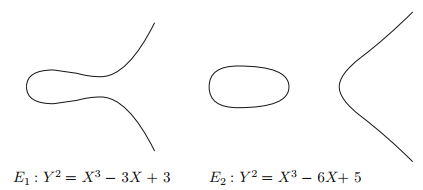
\includegraphics[scale=1]{../im1.png}
\caption{Hai ví dụ minh họa về đường cong elliptic}
\end{center}
\end{figure}
Một đặc điểm của đường cong elliptic là lấy hai điểm bất kì trên đường cong và cộng chúng lại để tạo ra một điểm thứ ba nằm trên đường cong. Nhưng không giống như luật cộng thông thường chúng ta sẽ mô tả luật cộng thông qua hình học.
\begin{figure}[h] \label{h2.2}
\begin{center}
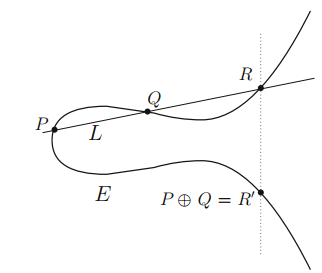
\includegraphics[scale=1]{../im2.png}
\caption{Luật cộng trên đường cong elliptic}
\end{center}
\end{figure}

Cho $P$ và $Q$ là hai điểm trên đường cong elliptic $E$, như hình \ref{h2.2}. Kẻ đường thẳng $L$ đi qua $P$ và $Q$. Đường thẳng $L$ cắt đường cong $E$ tại ba điểm, trong đố có hai điểm $P$ và $Q$ và một điểm khác là $R$. Chúng ta lấy điểm $R$ và chiếu nó theo chục x để lấy được điểm mới $R'$. Điểm $R'$ được gọi là "tổng của $P$ và $Q$", có thể thấy phép cộng này không giống như các phép cộng thông thường. Chúng ta có thể kí hiệu phép cộng bởi $\oplus$.
\begin{displaymath}
P \oplus Q = R'
\end{displaymath}

Một ví dụ về luật cộng. Cho đường cong $E$ có phương trình:
\begin{equation}
Y^2 = X^3 - 15X + 18 \label{2.1}
\end{equation}

Cho hai điểm $P = (7,16)$ và $Q = (1,2)$ nằm trên đường cong $E$. Đường thẳng $L$ đi qua hai điểm có phương trình:
\begin{equation}
L: Y = \frac{7}{3} - \frac{1}{3} \label{2.2}
\end{equation}
Để tìm được giao điểm của đường thẳng $L$ và đường cong $E$. Chúng ta sẽ thay phương trình \ref{2.2} vào \ref{2.1} Ta có:
\begin{displaymath}
\begin{aligned}
(\frac{7}{3}X - \frac{1}{3})^2 & = X^3 - 15X + 18, \\
\frac{49}{9}X^2 - \frac{14}{9}X + \frac{1}{9} & = X^3 - 15X + 18, \\
0 & = X^3 - \frac{49}{9}X^2 - \frac{121}{9}X + \frac{161}{9}
\end{aligned}
\end{displaymath}
Chúng ta cần tìm nghiệm của đa thức. Nhìn chung để tìm nghiệm của đa thức là khó. Tuy nhiên như chúng ta đã biết $L \cap E$ Tại hai điểm P và Q nên ta có hai là $X = 7$ và $X = 1$,vì thế chúng ta có thể dễ dàng tìm được nghiệm thứ ba còn lại:
\begin{displaymath}
X^3 - \frac{49}{9}X^2 - \frac{121}{9}X + \frac{161}{9} = (X - 7)\cdot(X - 1)\cdot(X + \frac{23}{9})
\end{displaymath}
vì vậy điểm thứ ba là giao điểm của $L$ và $E$ sẽ có tọa $\displaystyle X = -\frac{23}{9}$. Chúng ta sẽ tìm tọa đô Y theo X bằng cách thay X vào phương trình \ref{2.2} kết quả $\displaystyle R = (-\frac{23}{9}, -\frac{170}{27})$. Cuối cùng chúng ta sẽ chiếu $R$ theo chục tọa đô X đạt được 
\begin{displaymath}
P \oplus Q = (-\frac{23}{9}, \frac{170}{27}).
\end{displaymath} 

\begin{figure}[h] 
\begin{center}
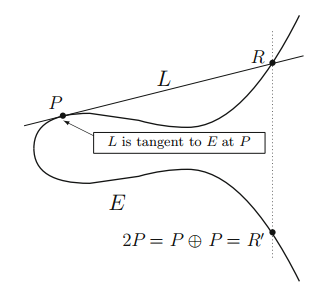
\includegraphics[scale=1]{../im3.png}
\caption{Cộng điểm P với chính nó} \label{h2.3}
\end{center}
\end{figure}

Có một số vấn đề, đầu tiên ta có thể nhìn thấy trong hình \ref{h2.2} nếu như $Q$ tiệm cận đến $P$ hay nói các khác là ta thực hiện phép cộng điểm $P$ với chính nó. Khi đó đường thẳng $L$ trở thành tiếp tuyến của $E$ tại $P$ thấy hình \ref{h2.3}. Do đó việc thực hiện phép cộng điểm $P$ với chính nó chúng ta chỉ đơn gian là kéo dài tiếp tuyến $L$ tại $P$ cắt $E$ tại $P$ và một điểm còn lại là $R$ và chúng ta vẫn xử lý như trước. Theo một nghĩa nào đó $L$ vẫn cắt $E$ tại 3 điểm nhưng điểm $P$ được tính là hai.

Ví dụ tiếp tục với đường cong E với phương trình \ref{2.1} và điểm P ở ví dụ trên, chúng ta sẽ tính $P \oplus P$ hệ số góc tiếp tuyến của $E$ ở $P$ được tính bởi đạo hàm phương trình \ref{2.1}. Do đó ta có:
\begin{displaymath}
2Y\frac{dY}{dX} = 3X^2 - 15 \Rightarrow \frac{dY}{dX} = \frac{3X^2 - 15}{2Y}
\end{displaymath}
Thay tọa độ điểm $P = (7,16)$ vào ta được hệ số góc $\lambda = \frac{33}{8}$ và đường thẳng tiếp tuyến với $E$ tại $P$ có phương trình
\begin{equation}
L: Y = \frac{33}{8}X - \frac{103}{8} \label{2.3}
\end{equation}
Từ \ref{2.3} và \ref{2.1} ta có:
\begin{displaymath}
\begin{aligned}
(\frac{33}{8}X - \frac{103}{8})^2 & = X^3 - 15X + 18, \\
X^3 - \frac{1089}{64}X^2 + \frac{2919}{32}X - \frac{9457}{64} & = 0, \\
(X - 7)^2\cdot(X - \frac{193}{64}) & = 0.
\end{aligned}
\end{displaymath}
Tọa độ $X$ của điểm P là nghiệm kép của phương trình ta dễ dàng tìm được nghiệm còn lại $\displaystyle X = \frac{193}{64}$, thay $X$ vào \ref{2.3} tìm được $\displaystyle Y = -\frac{223}{512}$.Từ đó ta thu được kết quả của phép cộng
\begin{displaymath}
P \oplus P = (\frac{193}{64}, \frac{223}{512}).
\end{displaymath}

\begin{figure}[h]
\begin{center}
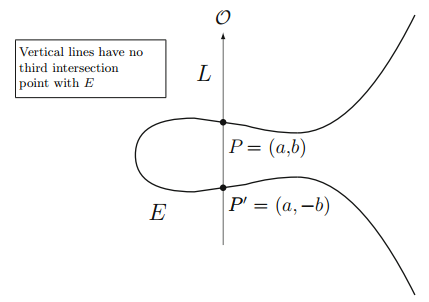
\includegraphics[scale=1]{../im4.png} \label{h2.4}
\caption{Đường thẳng đứng $L$ đi qua $P = (a, b)$ và $P' = (a, -b)$}
\end{center}
\end{figure}

Vấn đề thứ hai với luật cộng phát sinh là nếu như chúng ta cộng điểm $P = (a, b)$ với điẻm đối của nó  $P' = (a, -b)$ đường thẳng đi qua $P$ và $P'$ là x = a và nó chỉ cắt đường cong tại 2 điểm $P$ và $P'$(hình \ref{h2.4}) không có điểm thứ ba xuất hiện chúng ta sẽ thêm một điểm $O$ nằm ở vô cùng và điểm này không tồn tại trong mặt phẳng XY, chúng ta giả định nó luôn nằm trên đường thẳng dọc và chúng ta sẽ xét phép cộng như sau
\begin{displaymath}
P \oplus P' = O.
\end{displaymath}

Nếu công điểm $O$ với điểm $P$ nằm trên E sẽ như nào? Đường thẳng $L$ đi qua $O$ và $P$ là đường theo chiều dọc đi qua $P$ khi đó $O$ nằm trên đường dọc này và đường thẳng sẽ cắt $E$ tại điểm $P$, $O$ và điểm $P' = (a , -b)$. Nên phép công $P$ với $O$, chúng ta lấy hình chiếu của $P'$ qua trục X sẽ thu được điểm $P$ ban đầu. Nói một các khác $P \oplus O = P$, vì vậy $O$ giống như số không trong phép cộng của đường cong elliptic

Qua đây có một số định nghĩa về đường cong elliptic
\\[6pt]
\begin{definition}
Một đường cong $E$ là tập các nghiệm của phương trình Weierstrass
\begin{displaymath}
E: Y^2 = X^3 + AX + B,
\end{displaymath}
cùng với điểm $O$, với hằng số A, B thỏa mãn điều kiện
\begin{displaymath}
4A^3 + 27B^2 \neq 0,
\end{displaymath}
\end{definition}

Luật cộng trên $E$ được định nghĩa như sau. Cho $P$ và $Q$ là hai điểm trên $E$. Cho $L$ là đường thẳng qua $P$ và $Q$, hoặc là tiếp tuyến của $E$ tại $P$ nếu như $P = Q$. Giao điểm của $E$ và $L$ có chứa ba điểm $P, Q, R$ phép cộng sẽ được tính thích hợp với điểm $O$ nằm trên đường dọc vô cùng. Điểm $R = (a, b)$, tổng của $P$ và $Q$ được định nghĩa là $R' = (a, -b)$ hình chiếu của $R$ qua trục X. Tổng này được định nghĩa là $P \oplus Q$ hay đơn gian hơn là $P + Q$.

Hơn nữa, nếu $P = (a, b)$ chúng ta định nghĩa điểm đối $-P = (a, -b)$, chúng ta định nghĩa $P - Q$ trở thành $P + (-Q)$. Tương tự phép cộng lặp nhiều lần được biểu diễn như phép nhân một điểm với một số nguyên,
\begin{displaymath}
nP = \underbrace{P + P + P + \ldots + P}_{n}.
\end{displaymath}
\begin{theorem} \label{dl2.1}
Cho đường cong $E$. Luật cộng trên đường cong $E$ thỏa mãn tính chất:
\begin{itemize}
\item[(a)] $P + O = O + P = P \ \forall P \in E$ (phần tử đơn vị)
\item[(b)] $P + (-P) = O \ \forall P \in E$ (phần tử nghịch)
\item[(c)] $(P + Q) + R = P + (Q + R) \ \forall P, Q, R \in E$ (kết hợp)
\item[(d)] $P + Q = Q + P \ \forall P, Q \in E$ (giao hoán) 
\end{itemize}
Hay nói cách khách tập các điểm thuôc $E$ với luật cộng tạo thành nhóm abelian
\end{theorem}
\begin{theorem} \label{dl2.2}
Thuật toán Cộng trên đường cong elliptic với phương trình đường cong Weierstrass. Cho
\begin{displaymath}
E: Y^2 = X^3 + AX + B
\end{displaymath}
là một đường cong elliptic và hai điểm $P_1$ và $P_2$ nằm trên đường cong $E$.
\begin{itemize}
\item[(a)] Nếu $P_1 = O$ thì $P_1 + P_2 = P_2$.
\item[(b)] trái lại $P_2 = 0$ thì $P_1 + P_2 = P_1$.
\item[(c)] trái lại $P_1 = (x_1, y_1)$ và $P_2 = (x_2, y_2)$
\item[(d)] nếu $x_1 = x_2$ và $y_1 = -y_2$ thì $P_1 + P_2 = O$.
\item[(e)] trái lại, định nghĩa $\lambda$ bằng
\begin{displaymath}
\lambda = \left\{ \begin{array}{ll}
\displaystyle \frac{y_2 - y_1}{x_2 - x_1} & if \ P_1 \neq P_2  \\
\\
\displaystyle \frac{3x_1^2 + A}{2y_1} & if \ P_1 = P_2,
\end{array} \right.
\end{displaymath}
và
\begin{displaymath}
x_3 = \lambda^2 - x_1 - x_2 \ \ \& \ \ y_3 = \lambda(x_1 - x_3) - y_1
\end{displaymath}
Phép cộng $P_1 + P_2 = (x_3,y_3)$
\end{itemize}
\end{theorem}
\subsection*{Đường cong Elliptic trên trường hữu hạn}
Trong phần trước chúng ta đã xem xét lí thuyết về đường cong bằng hình học. Ví dụ tổng của hai điểm phân biệt $P$ và $Q$ trên đường cong $E$ được định nghĩa bởi đường thẳng $L$ đi qua hai điểm $P$ và $Q$ sau đó tìm điểm thứ ba là giao điểm của $L$ và $E$ như minh họa hình[?]. Tuy nhiên để áp dụng lí thuyết elliptic vào mật mã, chúng ta cần nhìn đường cong và các điểm của nó có tọa độ nằm trong trường hữu hạn $F_p$ điều này dễ làm.
\begin{definition}
Cho $p$ $\geq$ 3 là một số nguyên tố. Một đường cong elliptic trên trường $F_p$ có công thức
\begin{center}
$E: Y^2 = X^3 + AX + B$ với $A, B \in F_p$ thỏa mãn $4A^3 + 27B^2 \neq  0$.
\end{center} 
Với tập các điểm trên E với tọa độ nằm trong trường $F_p$
\begin{center}
$E(F_p) = \{ (x, y): x, y \in F_p$ thỏa mãn $y^2 = x^3 + Ax + B \} \cup \{ O \}$
\end{center}
\end{definition}
Xem xét ví dụ với đường cong elliptic
\begin{center}
$E: Y^2 = X^3 + 3X + 8$ trên trường $F_{13}$
\end{center}
Chúng ta có thể tìm thấy các điểm của $E(F_{13})$ bằng các thay lần lượt các giá trị của $X = 0, 1, 2, \ldots, 12$ và kiểm tra với giá trị $X$ kết quả của phương trình $X^3 + 3X + 8$ có phải là một bình phương với modulo 13 không. Ví dụ thay $X = 0$ cho kết quả là 8 và 8 không phải là bình phương với modulo 13. Tiếp theo $X = 1$ cho kết quả 12 và 12 là căn bậc hai của modul 13.
\begin{center}
$5^2 \equiv 12 (mod 13)$ và $8^2 \equiv 12 (mod 13)$ trên trường $F_13$
\end{center}
Điều này sẽ cho hai điểm $(1, 5)$ và $(1, 8)$ trong trường $F_{13}$. Tiếp tục tính với các giá trị $X$ ta thu được danh sách các điểm.
\begin{displaymath}
E(F_{13}) = \{ O, (1, 5), (1, 8), (2, 3), (2, 10), (9, 6), (9, 7), (12, 2), (12, 11)\}
\end{displaymath}
Giả sử chúng ta có hai điểm $P = (x_1, y_1)$ và $Q = (x_2, y_2)$ là hai điểm nằm trên $e(F_p)$. Chúng ta sẽ định nghĩa phép cộng $P + Q$ là điểm có tọa độ $(x_3, y_3)$ thực hiện phép toán cộng(định lý \ref{dl2.2}). Chú ý rằng thuật toán này chỉ sử dụng các phép toán cộng, trừ , nhân ,chia liên quan đến các hệ số của đường cong $E$ và các điểm $P$ và $Q$. Khi các hệ số và tọa đô nằm trong trường $F_p$, chúng ta sẽ có điểm $(x_3, y_3)$ với tọa độ trong trường $F_p$.
\begin{theorem}
Cho $E$ là một đường cong trên trường $F_p$ và hai điểm $P$ và $Q$ nằm trong $E(F_p)$.
\begin{itemize}
\item[(a)] Thuật toán cộng đường cong elliptic (định lý \ref{dl2.2}) áp dụng với $P$ và $Q$ tạo điểm trong $E(F_p)$. Chúng ta định nghĩa $P + Q$.
\item[(b)] Luật cộng trên $E(F_p)$ thỏa mãn tất cả các tính chất của định lí \ref{dl2.1}. Hay nói cách khác luật cộng $E(F_p)$ nằm trong một nhóm hữu hạn phần tử. 
\end{itemize}
\end{theorem}
Xét ví dụ thuật toán cộng (định lí \ref{dl2.2}) với hai điểm $P = (9, 7)$ và $Q = (1, 8)$ trong $E(F_{13})$. Bước thứ e của thuật toán sẽ được tính đầu tiên
\begin{displaymath}
\lambda = \frac{y_2 - y_1}{x_2 - x_1} = \frac{8 - 7}{1 - 9} = \frac{1}{-8} = \frac{1}{5}	= 8,
\end{displaymath}
Ở đây các phép tính được thực hiện trên trường $\mathbb{F}_{13}$ vì vậy -8 = 5 và $\frac{1}{5} = 5^{-1} = 8$. Tiếp theo tính 
\begin{displaymath}
\vartheta = y_1 - \lambda x_1 = 7 - 8\cdot 9 = -65 = 0
\end{displaymath}
Cuối cùng phép cộng sẽ có kết quả
\begin{center}
\begin{tabular}{ll}
$x_3$ & = $\lambda^2 - x_1 - x_2 = 64 - 9 - 1 = 54 = 2$, \\
$y_3$ & = $-(\lambda x_3 + v) = -8\cdot2 = -16 = 10$
\end{tabular}
\end{center}
Hay $P + Q = (1, 8) + (9, 7) = (2, 10)$ in  $E(F_{13})$. Tương tự ta có thể tính thuật toán cộng $P = (9, 7)$ với chính nó. Tính
\begin{center}
$\displaystyle \lambda = \frac{3x_1^2 + A}{2y_1} = \frac{3\cdot9^2 + 3}{2\cdot7} = \frac{246}{14} = 12$ \ và \ $\vartheta = y_1 - \lambda x_1 = 7 - 12\cdot9 = 3$
\end{center}
Ta có kết quả là 
\begin{center}
$x_3 = \lambda^2 - x_1 - x_2 = (12)^2 - 9 - 9 = 9$ và $y_3 = -(\lambda x_3 + v) = -(12\cdot9 + 3) = 6$,
\end{center}
vì vậy $P + P = (9, 7) + (9, 7) = (9,6)$ trong trường $E(\mathbb{F}_{13})$
\subsection*{Thuật toán Double-and-Add}
Xuất phát từ việc khó phục hồi lại giá trị của n từ điểm $P$ và $Q = n\cdot P$ trong $E(\mathbb{F}_{p})$ đây là vấn đề khó của ECDLP. Tuy nhiên để sử dụng
\begin{displaymath}
\mathbb{Z} \rightarrow E(\mathbb{F}_p), \ \ \ n \mapsto nP,
\end{displaymath}
cho mật mã, chúng ta cần thực hiện phép tính $nP$ hiệu quả khi biết giá trị của $n$ và $P$. Nếu như $n$ lớn thì chúng ta chẳng muốn tính $nP$ bằng cách $P, 2P, 3P, 4P, \ldots .$
Các toán tử sử dụng trong tính toán đường cong elliptic được viết như phép cộng vì thế chúng ta sẽ gọi nó là "doubling-and-add". Ý tưởng cơ bản của thuật toán là chúng ta sẽ phân tích số n thành biểu diễn nhị phân
\begin{center}
$n = n_0 + n_1\cdot2 + n_2\cdot4 + n_3\cdot8 + \ldots + n_r\cdot2^r$ với $n_0, n_1, \ldots , n_r \in \{0, 1\}$.
\end{center}
Nếu chúng ta giả sử $n_r = 1$. Chúng ta có thể tính
\begin{displaymath}
Q_0 = P, \ \ Q_1 = 2Q_0, \ \ Q_2 = 2Q_1, \ldots , Q_r = 2Q_{r - 1}.
\end{displaymath}
Chú ý rằng $Q_i$, đơn giản chỉ là gấp hai lần $Q_{i-1}$ vì vậy 
\begin{displaymath}
Q_i = 2^iP.
\end{displaymath}
Các điểm là được biểu diễn như là phép với một số mũ cơ số 2, tính toán các điểm này yêu cầu r phép doubling. Cuối cùng chúng ta tính được $nP$ sử dụng r phép cộng
\begin{displaymath}
nP = n_0Q_0 + n_1Q_1 + n_2Q_2 + \ldots + n_rQ_r.
\end{displaymath}
Do đó tổng thời gian tính toán $nP$ tối đa là 2r phép toán trong $E(\mathbb{F}_p)$. Chú ý rằng $n \geq 2^r$, vì vậy không lớn hơn $2\log_2(n)$ phép toán để tính $nP$. Điều này tạo nên sự linh hoạt khi tính $nP$ thậm trí cả khi giá trị của n là lớn. Thuật toán tổng quát Double-and-Add.
\begin{algorithm}[H]
\caption{The double-and-add algorithm for elliptic curves}
\textbf{Input:} Điểm P nằm trường elliptic và số nguyên n >= 1
\begin{algorithmic}[1]
\State $Set \ Q = P \ and \  R = O$.
\State Loop while $n > 0$
\State \ \ \ \ If $n \equiv 1$ (mod 2), set $R = R + Q$.
\State \ \ \ \ $Q = 2Q$ and $n = \lfloor n/2 \rfloor$.
\State \ \ \ \ If $n > 0$, continue with loop at Step 2.
\State Return the point $R$, which equals $nP$.
\end{algorithmic}
\end{algorithm}
%\subsection*{Hệ tọa độ}
%Trong phương trình đường cong tổng quát xem xét hai tọa độ x và y. Ví dụ: xem xét đường cong Montgomery trên trường F được xác định bởi:
%\begin{center}
%$By^2 = x^3 + Ax^2 + x$ \ \ \ \  $A, B \in F$ và $B(A^2 - 4) \neq 0$
%\end{center}
%A, B là các hằng số xác định đường cong. Phần tử trên đường cong là cặp tọa độ (x, y). Tuy nhiên có thể biểu diễn mở rộng theo bảng sau:
%\begin{center}
%\begin{tabular}{rll}
%$(x ,y)$ & affine	 \\
%$(X, Y, Z, ZZ)$ & standard & với $x = X/Z$ và $y = Y/Z$ và %$ZZ = Z^2$ \\
%$(X, Y, Z)$ & projective & với $x = X/Z$ và $y = Y/Z$ \\
%$(X, Y, Z)$ & Lopez-Dahab & với $x = X/Z$ và $y = Y/Z^2$ \\
%$(X, Y, Z)$ & Jacobian & với $x = X/Z^2$ và	$y = Y/Z^3$ \\
%$(X, Y, Z, Z^2, XZ )$ & Extended Lopez-Dahab & với $x = X/Z$ và $y = Y/Z^2$ \\
%$(X, Y, Z, Z^2)$ &  Extended Jacobian & với $x = X/Z^2$ và %$y = Y/Z^3$ \\
%$(X, Y, Z, T)$ & Extended Twisted Edwards & với $x = X/Z and Y = Y/Z$ với $T = X \cdot Y$ 
%\end{tabular}
%\end{center}
%\subsection*{Weierstrass curve}
\subsection*{Montgomery curve}
Trong toán học những đường cong Montgomery là một dạng của đường cong elliptic , khác với Weierstrass , được giới thiệu bởi Peter L. Montgomery vào năm 1987. Nó được sử dụng cho một số tính toán nhất định, và đặc biệt trong mật mã ứng dụng khác nhau.

Một đường cong Montgomery trên trường $\mathbb{K}$ được định nghĩa bởi phương trình 
\begin{displaymath}
M_{A,B}: By^2 = x^3 + Ax^2 + x
\end{displaymath}
với điều kiện $A, B \in \mathbb{K}$ và với $B(A^2 - 4) \neq 0$. Đường cong này được xem xét trên một trường hữu hạn $\mathbb{K}$($\mathbb{K} = \mathbb{F}_q$) với hai đặc điểm khác như $A \in \mathbb{K} \setminus \{-2, 2\}, B \in \mathbb{K} \setminus\{0\}$
\subsubsection*{Luật cộng}
Cho hai điểm $P_{1} = (x_{1}, y_{1}), P_{2}=(x_{2},y_{2})$ trên đường cong Montgomery $M_{A, B}$ trong hệ tọa độ affine, điểm $P_{3} = P_{1} + P_{2}$ biểu diễn hình học, điểm thứ ba là giao điểm giữa $M_{A, B}$ và đường thẳng đi qua $P_{1}$ và $P_{2}$. Có thể tìm tọa độ $(x_3, y_3)$ của $P_{3}$, theo cách sau:
\begin{itemize}
\item[1, ] Xem xét một đường thẳng $y = lx + m$ trong mặt phẳng affine và để nó đi qua $P_{1}$ và $P_{2}$ (áp đặt điều kiện), theo cách này, người ta có được $\displaystyle{l = \frac {y_{2} - y_{1}}{x_{2} - x_{1}}}$ và $\displaystyle{m = y_ {1} - \left({\frac {y_ {2} -y_ {1}} {x_ {2} -x_ {1}}} \right)x_{1}}$
\item[2, ] giao của đường thẳng với đường cong $M_{A, B}$, thay thế $y$ biến trong phương trình đường cong với $y = lx + m$ phương trình thu được:
\begin{displaymath}
x^3 + (A - Bl^2)x^2 + (1 - 2Blm)x - Bm^2 = 0.
\end{displaymath}
Như đã được quan sát trước đây, phương trình này có ba giải pháp tương ứng với tọa độ x của $P_{1}$,$P_{2}$ và $P_{3}$. Đặc biệt phương trình này có thể được viết lại thành:
\begin{displaymath}
(x - x_1)(x - x_2)(x - x_3) = 0
\end{displaymath}
\item[3, ] So sánh các hệ số của hai phương trình giống hệt nhau đã nêu ở trên, đặc biệt là các hệ số của các số hạng thứ hai, thu được:
\begin{displaymath}
-x_1 - x_2 - x_3 = A - Bl^2
\end{displaymath}
Vì thế, $x_3$ có thể được viết dưới dạng $x_{1}$, $y_{1}$, $x_{2}$, $y_{2}$, như:
\begin{displaymath}
x_3 = B\left(\frac{y_2 - y_1}{x_2 - x_1} \right)^2 - A - x_1 - x_2
\end{displaymath}
\item[4, ] Để tìm tọa độ y của điểm $P_{3}$, thay thế giá trị $x_{3}$ vào đường thẳng $y = lx + m$. Lưu ý rằng điều này sẽ không cho điểm $P_{3}$ trực tiếp. Thật vậy, với phương pháp này ta tìm thấy tọa độ của điểm $R$ sao cho $R + P_1 + P_2 = P_\infty$, nhưng  kết quả cần là tổng giữa $P_{1}$ và $P_{2}$, thì cần phải quan sát rằng: $R + P_1 + P_2 = P_\infty$ nếu và chỉ nếu $-R = P_1 + P_2$. Vì vậy, cho điểm $R$, nó là cần tìm $-R$, nhưng điều này có thể được thực hiện dễ dàng bằng cách thay đổi dấu y tọa độ của $R$. Nói cách khác, nó sẽ là cần thay đổi dấu của y bằng cách thay thế giá trị  $x_{3}$ trong phương trình đường thẳng.
Tóm lại tọa độ của điểm $P_3 = (x_3, y_3), P_3 = P_1 + P_2$ là:
\begin{displaymath}
x_3 = \frac{B(y_2-y_1)^2}{(x_2-x_1)^2}-A-x_1-x_2=\frac{B(x_2y_1-x_1y_2)^2}{x_1x_2(x_2-x_1)^2}
\end{displaymath}
\begin{displaymath}
y_3 = \frac{(2x_1+x_2+A)(y_2-y_1)}{x_2-x_1}-\frac{B(y_2-y_1)^3}{(x_2-x_1)^3}-y_1
\end{displaymath}
\end{itemize}
\subsubsection*{Doubling}
Cho một điểm $P_{1}$ trên đường cong Montgomery $M_{A, B}$, điểm $[2]P_1$ đại diện cho điểm hình học của điểm giao nhau thứ ba giữa đường cong và đường tiếp tuyến tại $P_{1}$; vì vậy, để tìm tọa độ của điểm $P_3 = 2P_1$, trong trường hợp này, đường thẳng $y  =  lx  +  m$ phải tiếp xúc với đường cong tại $P_{1}$, do đó, nếu $M_{A, B}: f(x, y) = 0$ với
\begin{displaymath}
f(x, y) = x^3 + Ax^2 + x - By^2
\end{displaymath}
giá trị của l biểu diễn hệ số góc của đường thẳng, cho bởi:
\begin{displaymath}
 l=-\left.\frac{\partial f}{\partial x}\right/\frac{\partial f}{\partial y}
\end{displaymath}
Vì vậy $\displaystyle l = \frac{3x_1^2 + 2Ax_1 + 1}{2By_1}$ và tọa độ điểm $P_3,P_3 = 2P_1$ là:
\begin{displaymath}
{\displaystyle {\begin{aligned}x_{3}&=Bl^{2}-A-x_{1}-x_{1}={\frac {B(3x_{1}^{2}+2Ax_{1}+1)^{2}}{(2By_{1})^{2}}}-A-x_{1}-x_{1}\\&={\frac {(x_{1}^{2}-1)^{2}}{4By_{1}^{2}}}={\frac {(x_{1}^{2}-1)^{2}}{4x_{1}(x_{1}^{2}+Ax_{1}+1)}}\\[8pt]y_{3}&=(2x_{1}+x_{1}+A)l-Bl^{3}-y_{1}\\&={\frac {(2x_{1}+x_{1}+A)(3{x_{1}}^{2}+2Ax_{1}+1)}{2By_{1}}}-{\frac {B(3{x_{1}}^{2}+2Ax_{1}+1)^{3}}{(2By_{1})^{3}}}-y_{1}.\end{aligned}}}
\end{displaymath}
\subsection*{Edwards curve}
Trong toán học , các đường cong Edwards là một họ các đường cong elip được Harold Edwards nghiên cứu năm 2007. Khái niệm về các đường cong elliptic trên các trường hữu hạn được sử dụng rộng rãi trong mã hóa đường cong elip. Các ứng dụng của các đường cong Edwards tới mật mã được Bernstein và Lange phát triển : chúng đã chỉ ra một số ưu điểm của dạng Edwards so với dạng Weierstrass.

Phương trình của một đường cong Edwards trên một trường K mà không có đặc tính 2 là:
\begin{displaymath}
x^{2}+y^{2}=1+dx^{2}y^{2}
\end{displaymath}
cho một số vô hướng  $d \in K \setminus \{0,1\}$. Ngoài ra dạng sau với các tham số c và d được gọi là đường cong Edwards:
\begin{displaymath}
x^2 + y^2 = c^2(1 + dx^2y^2)
\end{displaymath}
trong đó $c, d \in K$ với $cd(1 - c^4\cdot d) \neq 0$ \\
Mỗi đường cong Edwards tương đương với đường cong elip ở dạng Weierstrass , và do đó thừa nhận luật nhóm đại số một khi ta chọn một điểm để phục vụ như là một phần tử trung lập. Nếu K là hữu hạn, thì một số lượng đáng kể tất cả các đường cong elliptic trên $K$ có thể được viết dưới dạng đường cong Edwards. Thông thường các đường cong elip ở dạng Edwards được xác định có c = 1, không mất tính tổng quát. Trong các phần sau, giả sử rằng c = 1.
\subsubsection{Luật cộng}
Trên bất kỳ đường cong elliptic nào, có một điểm gọi là phần tử đơn vị. Đối với đường cong Edwards, lấy phần tử trung tính là điểm (0, 1), tổng các điểm $(x_1,  y_1)$ và $(x_2 ,y_2)$ được đưa ra bởi công thức:
\begin{displaymath}
(x_1, y_1) + (x_2, y_2) = \left( \frac{x_1y_2 + x_2y_1}{1 + dx_1x_2y_1y_2}, \frac{y_1y_2 - x_1x_2}{1 - dx_1x_2y_1y_2} \right).
\end{displaymath}
Nghịch đảo của bất kì điểm nào $(x_1, y_1)$ là $(-x_1, y_1)$. Người ta kiểm tra rằng điểm $(0, -1)$ có cấp là 2, và điểm $(\pm 1, 0)$ có cấp là 4, Trong thưc tế, một đường cong Edward luôn luôn có một điểm có cấp là 4 với tọa độ trong trường $K$.
Nếu d không phải là một bình phương trong $K$ và $\displaystyle (x_{1}, y_{1}), (x_{2}, y_{2}) \in \{(x, y)|x^{2} + y^{2} = 1 + dx^{2}y^{2} \}$, không có điểm đặc biệt có mẫu số $1 +  dx_1x_2y_1y_2 và 1 -  dx_1 x_2y_1y_2$ bằng 0. Do đó, luật cộng Edwards là hoàn tất khi d không phải là một bình phương trong trường $K$. Điều này có nghĩa là các công thức sẽ làm việc tốt và không có lỗi với các phép toán doubling, phần tử đơn vị, phần tử âm. Nói cách khác, nó được định nghĩa cho tất cả các cặp điểm đầu vào trên đường cong Edwards trên $K$ và kết quả cho tổng của các điểm đầu vào.
Nếu $d$ là một bình phương $K$ , thì phép toán tương tự có thể có các điểm đặc biệt, tức là có thể có cặp $(x_1, y_1)$ và $(x_2, y_2)$ trong đó 1$ +  dx_1x_2y_1y_2 = 0$ hoặc $1 -  dx_1x_2y_1y_2 = 0$.
Một trong những tính năng hấp dẫn của luật cộng của Edwards là nó được thống nhất mạnh mẽ, tức là nó cũng có thể được sử dụng để gấp đôi một điểm, đơn giản hóa việc bảo vệ chống lại tấn công bên kênh. Công thức cộng ở trên nhanh hơn các công thức thống nhất khác và có tính chất hoàn chỉnh mạnh.
\subsubsection*{Doubling}
Doubling có thể được thực hiện với chính xác công thức tương tự như cộng. Doubling đề cập đến trường hợp trong đó các đầu vào $(x_1, y_1)$ và $(x_2, y_2)$ được biết là bằng nhau. Vì $(x_1, y_1)$ nằm trên đường cong Edwards, ta có thể thay thế hệ số bằng $(x_1^2 + y_1^2  - 1)/x_1^2y_1^2$ như sau:
\begin{displaymath}
{\begin{aligned}2(x_{1},y_{1})&=(x_{1},y_{1})+(x_{1},y_{1})\\[6pt]2(x_{1},y_{1})&=\left({\frac  {2x_{1}y_{1}}{1+dx_{1}^{2}y_{1}^{2}}},{\frac  {y_{1}^{2}-x_{1}^{2}}{1-dx_{1}^{2}y_{1}^{2}}}\right)\\[6pt]&=\left({\frac  {2x_{1}y_{1}}{x_{1}^{2}+y_{1}^{2}}},{\frac  {y_{1}^{2}-x_{1}^{2}}{2-x_{1}^{2}-y_{1}^{2}}}\right)\end{aligned}}
\end{displaymath}
Điều này làm giảm mức độ mẫu số từ 4 đến 2, được phản ánh trong doubling. Luật cộng chung trong các tọa độ Edwards mất $10M + 1S + 1C + 1D + 7a$ và chi phí phép doubling là $3M + 4S + 3C + 6a$. Trong đó M là phép nhân trường, S là các phép bình phương trong trường , D là chi phí nhân với một tham số đường cong có thể lựa chọn và một trường bổ sung.
\subsection*{Twisted Edwards curve}
Trong hình học đại số , các đường cong Twisted Edwards là mô hình mặt phẳng của các đường cong elip , một sự tổng quát của các đường cong Edwards được giới thiệu bởi Bernstein , Birkner, Joye, Lange và Peters trong năm 2008. Bộ đường cong được đặt tên theo nhà toán học Harold M. Edwards . Đường cong Elliptic rất quan trọng trong mật mã khóa công khai và các đường cong Twist Edwards nằm ở trung tâm của một lược đồ chữ ký điện tử gọi là EdDSA mang lại hiệu năng cao trong khi tránh các vấn đề bảo mật xuất hiện trong các chương trình chữ ký số khác.

Như tên cho thấy, mỗi đường cong Twist Edwards là một xoắn của một đường cong Edwards. Đường cong Twist Edwards $E_{a, d}$ trên một trường $\displaystyle \mathbb{K}$ trong đó có $\displaystyle \mathrm{char}(\mathbb{K}) \neq 2$ là một đường cong mặt phẳng affine được xác định bởi phương trình:
\begin{displaymath}
E_{E_{a,d}}: ax^2 + y^2 = 1 + dx^2y^2
\end{displaymath}
Ở đâu $a, d$ là các phần tử khác 0 của $\displaystyle \mathbb{K}$. Đường cong Edwards là đường cong Twist Edwards với a = 1.
Mỗi đường cong Twist Edwards đều tương đương với đường cong elip ở dạng Montgomery và ngược lại.
\subsubsection*{Luật cộng}
Cho $\displaystyle \mathbb{K}$ là một trường có đặc điểm là khác 2. Để $\displaystyle (x_{1}, y_{1})$ và $\displaystyle (x_{2}, y_{2})$ là điểm trên đường cong Twist Edwards. Phương trình của đường cong Twist Edwards được viết như:
\begin{displaymath}
E_{E,a,d}: ax^2 + y^2 = 1 + dx^2y^2.
\end{displaymath}
Tổng của $(x_1, y_1)$ và $(x_2, y_2)$ trên $E_{E,a,d}$ là:
\begin{displaymath}
(x_{1}, y_{1}) + (x_{2}, y_{2}) = \left({\frac {x_{1}y_{2} + y_{1}x_{2}} { 1 + dx_{1}x_{2}y_{1}y_{2}}}, {\frac{y_{1}y_{2} - ax_{1}x_{2}} {1 - dx_{1}x_{2}y_{1}y_{2}}} \right)
\end{displaymath}
Phần tử đơn vị là $(0,1)$ và âm của điểm $(x_1, y_1)$ là $(-x_1, y_1)$. Công thức này cũng làm việc với doubling. Nếu a là một bình phương trong $\mathbb{K}$ và d không phải bình phương trong $\mathbb{K}$, công thức trên là hoàn tất. Điều này có nghĩa là chúng ta có thể công thức cho tất cả các cặp điểm mà không xảy ra ngoai lệ.
\subsubsection*{Doubling}
Doubling có thể được thực hiện với chính xác công thức tương tự như phép cộng. Doubling một điểm $(x_1 , y_1)$ trên đường cong $E_{E,a,d}$ là: $[2](x_1, y_1) = (x_3, y_3)$ ở đây
\begin{displaymath}
\begin{aligned}
x_{3} &= {\frac{x_{1}y_{1}+y_{1}x_{1}}{1+dx_{1}x_{1}y_{1}y_{1}}}={\frac {2x_{1}y_{1}}{ax_{1}^{2}+y_{1}^{2}}} \\[6pt]
y_{3} &= {\frac {y_{1}y_{1} - ax_{1}x_{1}}{1 - dx_{1}x_{1}y_{1}y_{1}}}={\frac{y_{1}^{2} - ax_{1}^{2}}{2 - ax_{1}^{2} - y_{1}^{2}}}.
\end{aligned}
\end{displaymath}
\section{Mật mã dựa trên đường cong Elliptic}
Chúng ta bắt đầu với ứng dụng đơn giản nhất, trao đổi khóa Diffie – Hellman, ít liên quan đến việc thay thế vấn đề logarit rời rạc cho trường $\mathbb{F}_p$ hữu hạn với bài toán logarit rời rạc cho đường cong elip $E_(\mathbb{F}_p)$. Sau đó chúng ta sẽ mô tả các tương tự elliptic của hệ thống mã khóa công khai Elgamal và thuật toán chữ ký số (DSA).
\subsection*{Trao đổi khóa với Elliptic Diffie-Hellman}
Alice và Bob đồng ý sử dụng một đường cong elliptic đặc biệt $E_(\mathbb{F}_p)$ và một điểm cụ thể $P \in E_(\mathbb{F}_p)$. Alice chọn số nguyên $n_A$ bí mật và Bob chọn số nguyên $n_B$ bí mật. Họ tính toán các bội số liên quan
\begin{displaymath}
\overbrace{Q_A = n_AP}^{Alice} \ \ \ and \ \ \ \overbrace{Q_B = n_BP}^{Bob}
\end{displaymath}
và họ trao đổi các giá trị của $Q_A$ và $Q_B$. Sau đó Alice sử dụng hệ số bí mật của mình để tính toán $n_AQ_B$, và Bob tương tự tính toán $n_BQ_A$. Bây giờ họ có giá trị bí mật được chia sẻ
\begin{displaymath}
n_AQ_B = (n_An_B)P = n_BQ_A,
\end{displaymath}
mà họ có thể sử dụng như một chìa khóa để giao tiếp riêng tư thông qua một mật mã đối xứng. Tổng quát trao đổi khóa elliptic Diffie–Hellman
\begin{figure}[h]
\begin{center}
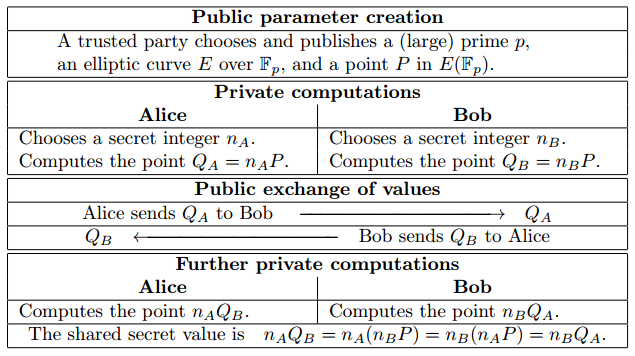
\includegraphics[scale=0.9]{../im7.png}
\caption{Trao đồi khóa Diffe-Hellman sử dụng đường cong elliptic}
\end{center}
\end{figure}
\subsection*{Hệ thống mã khóa công khai Elgamal}
Alice và Bob đồng ý sử dụng một số nguyên tố $p$ cụ thể, đường cong elliptic $E$ và điểm $P \in E(\mathbb{F}_p)$. Alice chọn một số nhân $n_A$ bí mật và điểm $Q_A = n_AP$ làm khóa công khai của cô ấy. Nội dung của Bob là một điểm $M \in E(\mathbb{F}_p)$. Anh ta chọn một số nguyên k là yếu tố ngẫu nhiên của anh ấy và các tính toán
\begin{displaymath}
\ \ \ \ C_1 = kP \ \ \ \ and \ \ \ \ C_2 = M + kQ_A.
\end{displaymath}
Anh ấy sẽ gửi hai điểm $(C_1, C_2)$ đến Alice và Alice sẽ tính:
\begin{displaymath} 
C_2 - n_AC_1 = (M + kQ_A) - n_A(kP) = M + k(n_AP) - n_A(kP) = M
\end{displaymath}
để phục hồi bản rõ. Tổng quát hệ mã khóa công khai Elgamal \\
\begin{figure}[h]
\begin{center}
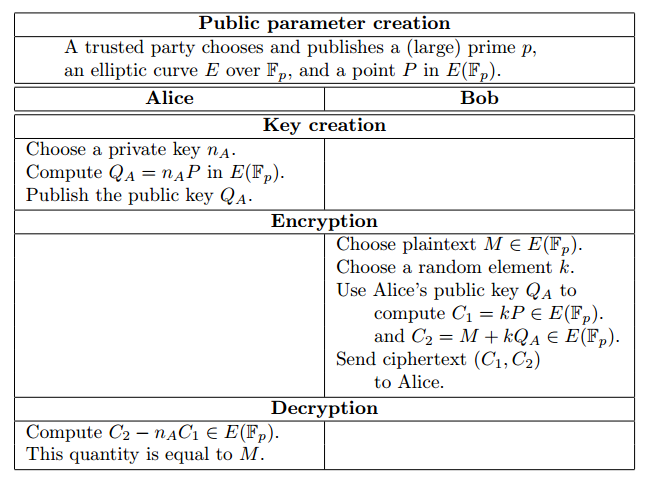
\includegraphics[scale=0.9]{../im5.png}
\caption{Tạo khóa, mã hóa, giải mã sử dụng Elliptic Elgamal}
\end{center}
\end{figure}
Trong thực tế, hệ mã khóa công khai Elgamal elliptic hoạt động tốt, nhưng có một số khó khăn thực tế
\begin{itemize}
\item[1, ] Không có cách rõ ràng để đính kèm các tin nhắn văn bản vào các điểm trong $E(\mathbb{F}_p)$
\item[2, ] Hệ thống mã hóa elgamal elliptic có hệ số mở rộng 4 đến 1, so với tỷ lệ mở rộng 2 đến 1 của Elgamal khi sử dụng $\mathbb{F}_p$.
\end{itemize}
Lý do elgamal elip có một mở rộng thông điệp 4 đến 1 nằm trong thực tế là bản rõ M là một điểm duy nhất trong $E(\mathbb{F}_p)$. Bản mã $(C_1, C_2)$ bao gồm bốn số modulo $p$, vì mỗi điểm trong $E(\mathbb{F}_p)$ có hai tọa độ. Các phương pháp khác nhau đã được đề xuất để giải quyết những vấn đề này. Khó khăn trong việc liên kết các bản rõ với các điểm có thể được phá vỡ bằng cách chọn M ngẫu nhiên và sử dụng nó làm mặt nạ cho bản rõ thô thực sự.
Với ví dụ Alice và Bob. Thật không may, vì Alice phải tính toán $C_2 - n_AC_1$ ,cô ấy cần các giá trị chính xác của cả hai tọa độ x và y của $C_1$ và $C_2$. Tuy nhiên, tọa độ x của một điểm xác định tọa độ y lên để thay đổi dấu, vì vậy Bob có thể gửi thêm một bit, ví dụ
\begin{displaymath}
\lambda = \left\{ \begin{array}{ll}
\displaystyle 0 & if \  0 \leq y \leq \frac{1}{2}p,\\
\\
\displaystyle 1 & if \ \frac{1}{2} < y < p
\end{array} \right.
\end{displaymath}
Theo cách này, Bob chỉ cần gửi các tọa độ x của $C_1$ và $C_2$, cộng thêm hai bit phụ. Ý tưởng này đôi khi được gọi là nén điểm.
\subsection*{Thuật toán chữ ký số với Elliptic}
Thuật toán chũ ký số với Elliptic được mô tả sau đây:\\
\begin{figure}[h]
\begin{center}
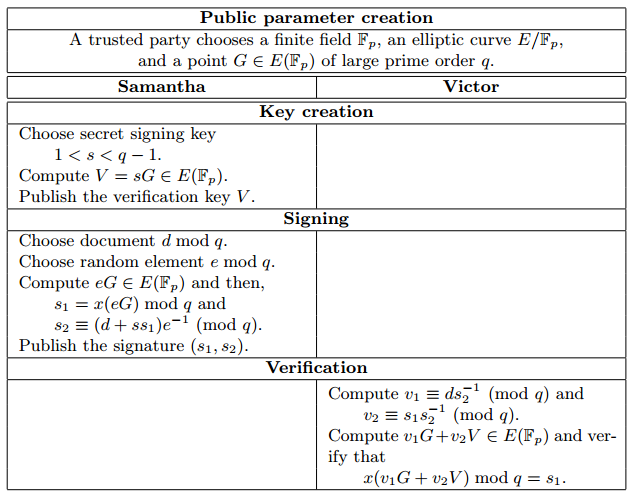
\includegraphics[scale=0.9]{../im6.png}
\caption{Chữ ký số ECDSA}
\end{center}
\end{figure}
tương tự như thuật toán chữ ký số đơn giản của DSA. ECDSA đang được sử dụng rộng rãi, đặc biệt là trong các tình huống mà kích thước chữ ký là quan trọng. \\

Để chứng minh rằng ECDSA hoạt động, tức là bước xác minh thành công trong việc xác minh chữ ký hợp lệ, chúng ta tính toán:
\begin{displaymath}
\begin{aligned}
v_1G + v_2V & = ds_2^{-1}G + s_1s_2^{-1}(sG) \\
            & = (d + ss_1)s_2^{-1}G \\
            & = (es_2)s_2^{-1}G \\
            & = eG \in E(\mathbb{F}_p).
\end{aligned}
\end{displaymath}
Do đó:
\begin{displaymath}
x(v_1G + v_2V) \mod \ q = x(eG)
\end{displaymath}
Chữ kí được chấp nhận là hợp lệ.
\chapter{Chứng thư số ẩn dựa trên đường cong Elliptic}
Trong chương này xác định sơ đồ chứng thư số ẩn của Elliptic Curve Qu-Vanstone (ECQV). Sơ đồ chứng thư số ẩn ECQV được xem như là một lược đồ chứng thư với mục đích chung cho các ứng dụng trong các hệ thống máy tính và truyền thông. Nó đặc biệt thích hợp cho các môi trường ứng dụng nơi có các tài nguyên như băng thông, sức mạnh tính toán và lưu trữ bị hạn chế. ECQV cung cấp giải pháp thay thế hiệu quả hơn cho chứng chỉ truyền thống.

Mục đích của chương này là để xem xét việc triển khai sơ đồ chứng thư số ẩn %ECQV. Việc triển khai có thể yêu cầu tuân thủ các sơ đồ mã hóa được chỉ định trong tài liệu này miễn là giao diện ngoài (đầu vào và đầu ra) cho các lược đồ tương đương với giao diện được chỉ định tại đây. Các tính toán nội bộ có thể được thực hiện như được chỉ định ở đây, hoặc có thể được thực hiện thông qua một chuỗi hoạt động tương đương.
\section{Hàm băm}
Hàm băm được sử dụng trong lược đồ ECQV để tính toán thông điệp của chứng chỉ được tạo hoặc xác minh. Hàm băm cũng được sử dụng trong việc tạo và xác thực tham số miền elliptic ngẫu nhiên một cách chính xác, và cũng có thể được sử dụng trong các quá trình tạo số ngẫu nhiên.

Mức độ bảo mật kết hợp với hàm băm phụ thuộc vào ứng dụng của nó. Trường hợp tránh xung đột là cần thiết, mức độ bảo mật tối đa bằng một nửa độ dài đầu ra (tính theo bit) của hàm băm. Trường hợp tránh xung đột là không cần thiết, mức độ bảo mật tối đa là độ dài đầu ra (tính theo bit) của hàm băm. Khả năng tránh xung đột nói chung là cần thiết để tính toán thông điệp cho chữ ký số.

Hàm băm được sử dụng bởi sơ đồ ECQV sẽ được chấp nhận hàm băm, như được chấp thuận trong mục đăng ký X9 00003, tiêu chuẩn băm an toàn (SHS). Mức độ bảo mật của hàm băm được phê duyệt được coi là tối đa một nửa độ dài đầu ra của nó cho các mục đích của tiêu chuẩn này. Danh sách một số hàm hăm tiêu chuẩn SHA-1, SHA-2, MD5, \ldots.

Hàm băm được sử dụng để tính toán chứng thư ẩn sẽ là hàm băm có mức bảo mật ít nhất là mức bảo mật của việc triển khai ECQV. Hàm băm được sử dụng cho các xác định tham số  elliptic sẽ là hàm băm có mức bảo mật là mức độ bảo mật của việc triển khai sơ đồ ECQV (ngoại trừ các xác định tham số elliptic ngẫu nhiên trong [SEC 2] được tạo bằng cách sử dụng SHA-1).
\section{Hàm băm một số nguyên modul n}
Trong nhiều bước của ECQV, một chuỗi octet(mỗi một ký tự trong xâu được biểu diễn bởi 8 bits) chiều dài tùy ý được băm bằng hàm băm mật mã H, và sau đó được chuyển đổi thành một số nguyên modulo n. Phần này chỉ định hàm kết quả, ký hiệu $H_n: \{0, 1,\ldots , 255\}^{*} \rightarrow [0,\ldots , n - 1]$, ánh xạ các chuỗi octet có độ dài tùy ý đến các số nguyên modulo n.
\begin{itemize}
\item[] \textbf{Input}
\begin{itemize}
\item[1. ] Một chuỗi octet có chiều dài tùy ý $S$.
\item[2. ] Hàm băm $H$ băm chuỗi octet chiều dài tùy ý thành các chuỗi bit dài của hashlen.
\item[3. ] Số nguyên $n$.
\end{itemize}
\item[] \textbf{Action}
\begin{itemize}
\item[1. ] Tính toán $h = H(S)$, một chuỗi bit dài hashlen bits.
\item[2. ] Lấy một số nguyên $e$ từ $h$ như sau:
\begin{itemize}
\item[2.1 ] Đặt E bằng $\lfloor log_2{n} \rfloor$ bits trái nhất của h.
\item[2.2 ] convert xâu bit $E$ thành xâu octect $E'$, sử dụng  Bit-String-to-Octet-String trong [SEC 1].
\item[2.3 ] convert xâu octect $E'$ thành số nguyên $e$ sử dụng Octet-String-to-Integer trong [SEC 1].
\end{itemize}
\end{itemize}
\item[] \textbf{Output} Số nguyên e, nằm trong khoảng $[0,\ldots , n - 1]$.
\end{itemize}
Lưu ý rằng nếu miền $H$ bị giới hạn ở kích thước tối đa thì miền $H_n$ bị hạn chế theo cùng một cách.
\section{Khởi tạo một số ngẫu nhiên}
Với tiêu chuẩn chứng thư số, tất cả các giá trị ngẫu nhiên phải được tạo bằng trình tạo số ngẫu nhiên được chấp thuận có mức độ bảo mật ít nhất là mức độ bảo mật của việc thực hiện ECQV. Trình tạo số ngẫu nhiên phải tuân thủ ANSI X9.82 hoặc NIST Special Publication 800-90A [NIST 800-90A]. Một bộ tạo số ngẫu nhiên phù hợp cũng được mô tả trong [SEC 1, 3.10]
\section{Các tham số khởi tạo và hợp lệ}
Việc tạo và xác nhận tham sốđường cong elliptic phải tuân theo [SEC 1].

Việc triển khai sử dụng cả ECQV lẫn các thuật toán ECC khác nên sử dụng điểm cơ sở ngẫu nhiên xác thực G, được xác định trong [SEC 2].


\section{Sơ đồ chứng thư số thực ECQV}
\subsection{Tổng quan}
Sơ đồ chứng chỉ số ẩn được sử dụng bởi ba thực thể - Tổ chức phát hành chứng chỉ
CA, người yêu cầu chứng chỉ U và bộ xử lý chứng chỉ V. Người yêu cầu U sẽ nhận được chứng chỉ số ẩn từ CA, xác nhận danh tính của U và cho phép V lấy khóa công khai của U. 
\begin{figure}[h]\label{h3.1}
\begin{center}
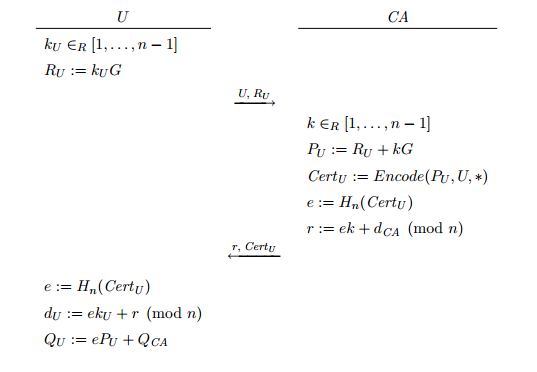
\includegraphics[scale=0.9]{../im8.png}
\caption{}
\end{center}
\end{figure}

Sơ đồ chứng thư số ẩn bao gồm sáu phần. Những phần này sẽ được sẽ được mô tả chi tiết.\\
\textbf{ECQV\_Setup}: Trong bước này, CA thiết lập các tham số đường cong elliptic, hàm băm, định dạng mã hóa chứng chỉ và tất cả các bên đã chọn một trình tạo số ngẫu nhiên. CA tạo ra một cặp khóa. Tất cả các bên phải nhận được bản sao xác thực các thông số và khóa công khai của CA. \\[6pt]
\textbf{Cert\_Request}: Người yêu cầu U phải tạo một yêu cầu cho một chứng chỉ, được gửi đến CA. Thành phần mật mã của yêu cầu là khóa công khai, được tạo ra bằng cách sử dụng cùng thủ tục như CA sử dụng trong khi thiết lập ECQV. \\ [6pt]
\textbf{Cert\_Generate}: Khi nhận được yêu cầu chứng chỉ từ U, CA xác nhận danh tính của U và tạo chứng chỉ số ẩn. CA gửi phản hồi cho U. \\ [6pt]
\textbf{Cert\_PK\_Extraction}: Với chứng chỉ số ẩn cho U người dùng, thông số và khóa công khai của CA, thuật toán trích xuất khóa công khai tính toán khóa công khai của U. \\ [6pt]
\textbf{Cert\_Reception}: Sau khi nhận được phản hồi cho yêu cầu chứng chỉ của mình, U đảm bảo tính hợp lệ của cặp khóa được chứng nhận ngầm

Cấp chứng thư là quy trình gồm hai bước, trong đó bước đầu tiên nhận được yêu cầu cấp chứng thư từ U và bước thứ hai là tạo phản hồi, chứa chứng thư. Hình \ref{h3.1} đã mô tả giao thức (thông tin).

Một số khác biệt giữa ECQV và chứng chỉ truyền thống liên quan đến việc ràng buộc giữa danh tính của người dùng và khóa công khai

Mộ
\subsection{Điều kiện tiên quyết: Cài đặt ECQV}
Tất cả các bên (CA nhà phát hành chứng thư, chủ sở hữu chứng thư U và bộ xử lý chứng thư V) sẽ phải thiết lập các điều kiện tiên quyết sau để sử dụng ECQV.
\begin{itemize}
\item[1, ] CA đã thiết lập một tập hợp các tham số EC để sử dụng với ECQV bao gồm $q, a, b, G, n$ và $h$. Các tham số phải được tạo bằng phương thức được chấp nhận chúng phải được đảm bảo tính hợp lệ trên EC và cung cấp mức độ bảo mật mong muốn(có thể tham khảo các phương thức tạo tham số hoặc các tham số sẵn có ở [SEC 1, 3.1] và [SEC 2]).
\item[2, ] CA đã chọn một hàm băm được chấp nhận với mức độ bảo mật mong muốn để sử dụng trong quy trình tạo chứng thư ECQV. Giả sử $H$ là hàm băm đã chọn và hashlen là độ dài của đầu ra hàm $H$. Như trong phần trước đã mô tả convert đâu ra của $H$ là một số nguyên dương n.
\item[3, ] CA và U chọn và khởi một số ngẫu nhiên đảm bảo được mức độ bảo mật mong muốn. Số ngẫu nhiên này được sử dụng để tạo khóa private trong quá trình yêu cầu chứng thư và quá trình tạo chứng thư.
\item[4, ] CA tạo được cặp khóa trên EC $(d_{CA}, Q_{CA})$ liên quan với các tham số EC được thiết lập từ ban đầu để sử dụng trong quá trình tạo chứng thư. Cặp khóa sẽ được tạo ra bằng cách sử dụng điểm  sinh và số ngẫu nhiên tạo ở mục 3(xem ở [SEC 1, §3.2.1]). CA sẽ đảm bảo tính hợp lệ của cặp khóa và sự đảm bảo của quyền sở hữu của khóa riêng (xem [SEC 1]).
\item[5, ] Chủ sở hữu $U$ của chứng thư cùng với bộ xử lý $V$ sẽ thu được tham số đường cong, hàm băm và khóa công khai của CA là $Q_{CA}$. U và V sẽ có một số đảm bảo sau:
\begin{itemize}
\item[5.1, ] Tính hợp lệ các tham số đường cong EC.
\item[5.2, ] Tính hợp lệ khóa công khai của CA, $Q_{CA}$
\item[5.3, ] Sở hữu khóa riêng, $d_{CA}$ của CA
\end{itemize}
\end{itemize}
\subsubsection{Mã hóa chứng thư} \label{subsec:3.5.2.1}
Mã hóa chứng chứng thư mô tả cách thông tin được thêm vào trong chứng thư phải được mã hóa dưới dạng chuỗi octet. Nó cũng chỉ định thông tin nào phải được thêm vào và thông tin nào là tùy chọn và mọi ràng buộc hoặc mối quan hệ giữa các phần của thông tin chứng thư.

Có ba kiểu mã hóa chứng thư(tham khỏa mô tả chi tiết xem ở[?])
\begin{itemize}
\item[•] \textbf{Fixed-length Fields}: là một mã hóa đơn giản, tối giản giúp đặt hiệu quả băng thông lên trước tất cả các mối quan tâm khác. Chứng chỉ bao gồm danh sách các trường, mỗi trường có độ dài cố định và định dạng được chia sẻ giữa tất cả các bên. Tiêu chuẩn này chỉ yêu cầu dữ liệu tái tạo khóa công khai PU là một trong các trường, để phần còn lại của định dạng mở cho người triển khai.
\item[•] \textbf{Minimal ASN.1 Encoding Scheme}: cũng được thiết kế để có hiệu quả băng thông. Đặc tả ASN.1 bao gồm các trường bắt buộc cơ bản và cho phép các phần mở rộng. Các trường cơ bản được đề xuất trong mã hóa này có độ dài cố định và do đó cũng có thể được sử dụng với định dạng độ dài cố định đơn giản hơn.
\item[•] \textbf{X.509-Compliant ASN.1 Encoding}: được thiết kế để bao gồm thông tin đầy đủ để cho phép chứng chỉ ECQV này được mã hóa lại dưới dạng chứng chỉ X.509 chuẩn.
\end{itemize}
\subsection{Yêu cầu chứng thư: Cert\_Request}
Người yêu cầu chứng chỉ U, sẽ sử dụng quy trình dưới đây để tạo yêu cầu chứng chỉ.
\begin{itemize}
\item[] \textbf{Input}
\begin{itemize}
\item[1. ] Các tham số đường cong EC được thiết lập bởi CA.
\item[2. ] Xâu biểu diễn định danh của U.
\end{itemize}
\item[] \textbf{Actions}
\begin{itemize}
\item[1. ] Khởi tạo cặp khóa $(k_u, R_u)$  trên EC liên quan tới các tham số được thiết lập với đường cong(tham khảo cách tạo cặp khóa ở [SEC 1, 3.2.1])
\item[2. ] Convert $R_u$ thành xâu octet $RU$ sử dụng  Elliptic-Curve-Point-to-Octet-String trong [SEC 1, 2.3]
\end{itemize}
\item[] \textbf{Output} khóa $k_U$ và yêu cầu chứng thư $(U, RU)$.
\end{itemize}

Giá trị $RU$ cùng với danh tính được định nghĩa $U$, tạo thành nội dung của yêu cầu chứng chỉ. Giá trị $k_U$ là bắt buộc trong các bước tương lai (để tính toán khóa riêng) và phải được giữ riêng tư. Yêu cầu chứng chỉ sẽ được gửi tới CA bằng cách sử dụng phương pháp bảo toàn tính toàn vẹn dữ liệu của thông báo.
\subsection{Xử lý tạo chứng thư: Cert\_Generate}
$CA$ sẽ sử dụng quy trình dưới đây để tạo ra một chứng thư và dữ liệu đóng góp khóa cá nhân để đáp ứng với một Cert\_Request từ $U$. Giả sử rằng $CA$ đã nhận được $U$, và $RU$ theo cách được xác thực và đã quyết định cấp chứng chỉ.
\begin{itemize}
\item[] \textbf{Input}
\begin{itemize}
\item[1. ] Các tham số đường cong EC được thiết lập bởi $CA$.
\item[2. ] Hàm băm được lựa chọn bơi $CA$.
\item[3. ] Khóa bí của $CA$, $d_{CA}$. 
\item[4. ] Một cái yêu cầu tạo chứng thư $(U, RU)$
\item[5. ] Phương thức mã hóa chứng thư (xem phần \ref{subsec:3.5.2.1})
\item[6. ] Các trường nhập bổ sung cho chứng thư.
\end{itemize}
\item[] \textbf{Actions}
\begin{itemize}
\item[1. ] Chuyển đổi chuỗi octet $RU$ thành một điểm trên đường cong elliptic bằng thuật toán chuyển đổi Octet-String-to-Elliptic Curve-Point(xem trong [SEC 1, §2.3.4]).
\item[2. ] Xác thực $RU$ bằng cách sử dụng kỹ thuật xác thực khóa công khai(xem ở [SEC 1, §3.2.2]). Nếu xác thực kết quả đầu ra là 'không hợp lệ' dừng lại.
\item[3. ] Tạo cặp khóa EC (k, kG) với các tham số đường cong elliptic đã được thiết lập. 
\item[4. ] Tính toán đường cong elliptic điểm $P_U = R_U + kG$
\item[5. ] Chuyển đổi $P_U$ sang chuỗi octet PU bằng cách sử dụng chuyển đổi Elliptic-Curve-Point-to-Octet-String [SEC 1]
\item[6. ] Mã hóa chứng thư với các trường nhập cần thiết và chuỗi octet PU như được chỉ ra
\item[7. ] Sự dụng hàm băm để tính $e = H_n(Cert_U)$ với modulo n.
\item[8. ] Nếu $eP_U + Q_{CA} = \mathcal{O}$, với $\mathcal{O}$ là điểm cơ sở, quay về bước 3.
\item[9. ] Tính số nguyên $r = ek + d_{CA} (mod \ n)$.
\end{itemize}
\item[] \textbf{Output} $(r, Cert_U)$, Ở đây $r$ là khóa đóng góp  và $Cert_U$ là chứng thư.
\end{itemize}

Phản hồi từ $CA$ có thể được công khai. Ngoài ra, nó có thể được truyền thông qua một kênh không an toàn, vì $U$ có thể xác minh rằng thông tin nhận được là hợp lệ. Để bảo mật, giá trị tạm thời $k$ phải được giữ riêng.

\subsection{Trích rút khóa công khai từ chứng thư: Cert\_PK\_Extraction}
Khóa công khai được liên kết với chứng thư được lấy từ chứng thư bằng khóa công khai của $CA$ và được khôi phục bằng quy trình sau. Bước này không yêu cầu bất kỳ thông tin bí mật nào và có thể được thực hiện bởi bất kỳ người dùng nào biết về $Cert_U$ và các tham số công khai được tạo bởi Thiết lập $ECQV$.
\begin{itemize}
\item[] \textbf{Input}
\begin{itemize}
\item[1. ] Các tham số đường cong EC được thiết lập bởi $CA$.
\item[2. ] Hàm băm $H$ được lựa chọn bởi $CA$.
\item[3. ] Khóa công khai của $Q_{CA}$.
\item[4. ] Chứng thư $Cert_U$.
\end{itemize}
\item[] \textbf{Actions}
\begin{itemize}
\item[1. ] Giải mã chứng thư $Cert_U$ theo các phương thức và các quy tắc giải mã chứng chỉ. Nếu giá trị trả lại là 'không hợp lệ' thì đầu ra 'không hợp lệ' và dừng lại, nếu không một chuỗi octet PU sẽ được trả lại.
\item[2. ] Chuyển đổi PU thành điểm $P_U$ bằng cách sử dụng chuyển đổi Octet-String-to-Elliptic-Curve-Point (xem [SEC 1, 2.3])
\item[3. ] Xác thực điểm $P_U$ sử dụng các kĩ thuật xác thực.
\item[4. ] Sử dụng hàm băm tính $e = H_n(Cert_U)$ với modulo $n$.
\item[5. ] Tính điểm $Q_U = eP_U + Q_{CA}$.
\end{itemize}
\item[] \textbf{Output} Hoặc là 'không hợp lệ' hoặc một public key $Q_U$
\end{itemize}
\subsection{Xử lý phản hồi cho yêu cầu chứng thư: Cert\_Reception}
Quy trình này xác thực nội dung của chứng thư ẩn và dữ liệu đóng góp khóa cá nhân do $CA$ cung cấp. Đầu ra của Cert\_PK\_Extraction và khóa riêng được tính ở đây, tạo thành một cặp khóa. Cert\_PK\_Extraction thực hiện kiểm tra tính hợp lệ của khóa công khai, vì vậy nó không được lặp lại ở đây. Người yêu cầu chứng chỉ $U$ sẽ sử dụng quy trình dưới đây, sau khi nhận được phản hồi yêu cầu chứng chỉ của họ, để tính toán khóa riêng cho đầu ra khóa công khai bằng Cert\_PK\_Extraction và xác nhận hợp lệ cặp khóa.
\begin{itemize}
\item[] \textbf{Input}
\begin{itemize}
\item[1. ] Các tham số đường cong EC được thiết lập bởi $CA$.
\item[2. ] Hàm băm $H$.
\item[3. ] Khóa riêng tạo bởi $U$, $k_U$.
\item[4. ] Đầu ra của Cert\_Generate: chứng thư $Cert_U$ và dữ liệu đóng góp khóa riêng, một số nguyên $r$.
\end{itemize}
\item[] \textbf{Actions}
\begin{itemize}
\item[1. ] Tính khóa công khai $Q_U$ sử dụng Cert\_PK\_Extraction .
\item[2. ] Sử dụng hàm băm để tính $e = H_n{Cert_U}$ vơi modulo n.
\item[3. ] Tính khóa bí mật $d_U = r + ek_U (mod \ n)$
\item[4. ] Tính $Q_U' = d_UG$.
\end{itemize}
\item[] \textbf{Output} 'hợp lệ' và $d_U$ nếu $Q_U = Q_U'$ nếu không 'không hợp lệ'.
\end{itemize}
\subsection{Sơ đồ tạo chứng chỉ tự ký ECQV}
\subsection{Trích rút khóa công khai từ chứng thư tự ký ECQV}
\chapter{Cài đặt cho thiết bị IoT}
\chapter*{Kết luận và hướng phát triển}
\begin{thebibliography}{9}
\bibitem{csattt} Sách Giáo trình Cơ sở An toàn Thông tin thầy Nguyễn Văn Khanh - Đại học Bách Khoa.
\end{thebibliography}

\end{document}